\chapter{Cài đặt hệ thống}\label{chap:implementation}

Chương này trình bày việc cài đặt các thiết kế ở \cref{chap:design}. Sau phần môi trường và cấu trúc mã nguồn, chương lần lượt mô tả ứng dụng iOS, máy chủ NestJS (xác thực, đặt phòng, thanh toán), bảng điều khiển React, thành phần gợi ý và việc triển khai. Các đoạn mã được trích trực tiếp từ kho mã nguồn theo số dòng, nên có thể đối chiếu chính xác.

\section{Môi trường phát triển}\label{sec:env}

\Cref{tab:env} liệt kê môi trường dùng để phát triển, kiểm thử và chụp ảnh giao diện trong báo cáo.

\begin{table}[H]
\centering
\caption{Môi trường phát triển và kiểm thử}\label{tab:env}
\begin{rtable}
\begin{tabular}{|L{4.2cm}|L{10.5cm}|}
\hline
\thead{Thành phần} & \thead{Cấu hình} \\ \hline
Máy phát triển & MacBook Pro Apple M2 Pro, 16 GB RAM, macOS 26.2 \\ \hline
iOS & Xcode 26.5; Simulator iPhone 17 Pro; iOS deployment target 26.2 \\ \hline
Máy chủ & Node.js 24 khi phát triển, Node.js 20 (Alpine) trong container triển khai; NestJS 11.2 \\ \hline
Cơ sở dữ liệu kiểm thử & MongoDB 7.0 chạy bằng Docker dưới dạng replica set một nút (cổng 27018) \\ \hline
Bảng điều khiển & Vite 5.4 dev server; Google Chrome headless để chụp ảnh ở ba kích thước màn hình \\ \hline
Nghiên cứu ML & Python 3.11.6 trong môi trường ảo \code{research/venv}; LightGBM 4.7.0 \\ \hline
Quản lý mã nguồn & Git, kho \code{github.com/NguyenDuyHieu49/Hotelia} \\ \hline
\end{tabular}
\end{rtable}
\end{table}

\section{Cấu trúc mã nguồn}\label{sec:source-tree}

Kho mã là một monorepo gồm năm thành phần (\cref{tab:source-tree}). Số dòng được đếm trên các tệp mã nguồn, không tính thư viện bên ngoài.

\begin{table}[H]
\centering
\caption{Cấu trúc kho mã nguồn}\label{tab:source-tree}
\begin{rtable}
\begin{tabular}{|L{3.4cm}|L{6.8cm}|C{2.0cm}|C{2.0cm}|}
\hline
\thead{Thư mục} & \thead{Nội dung} & \thead{Số tệp} & \thead{Số dòng} \\ \hline
\code{DuLich/} & Ứng dụng iOS (App, Core, Assets, Localizable.xcstrings) & 62 tệp Swift & 7.738 \\ \hline
\code{backend/src/} & Máy chủ NestJS: 12 module, \code{common}, cấu hình & 75 tệp TS + 13 tệp kiểm thử & 4.437 (không tính kiểm thử) \\ \hline
\code{backend/scripts/}, \code{data/} & Kịch bản di trú danh mục, kiểm thử MongoDB thật; dữ liệu nguồn JSON & 11 kịch bản & -- \\ \hline
\code{hotelia-dashboard/src/} & Bảng điều khiển React + TypeScript & 31 & 3.011 \\ \hline
\code{research/} & Huấn luyện LightGBM, xuất danh mục, thí nghiệm Trivago, 80 kiểm thử pytest & 11 tệp Python (scripts) & 2.702 \\ \hline
\code{docs/} & Tài liệu thiết kế: gợi ý, payOS, đăng nhập liên kết, bảo mật & 7 & -- \\ \hline
\end{tabular}
\end{rtable}
\end{table}

Ứng dụng iOS được tổ chức theo tính năng. Thư mục \code{App/} chứa phần dùng chung: xác thực (\code{Auth}), mạng (\code{Network/APIClient.swift}), bảo mật (\code{Security/SecureTokenStore.swift}), bản địa hóa (\code{Localization/AppLanguage.swift}) và hệ thống thiết kế (\code{Theme}). Thư mục \code{Core/} chứa các tính năng: \code{Explore}, \code{Booking}, \code{Profile}, \code{Admin} (màn hình chủ khách sạn và quản trị trên iOS), \code{Models}, \code{TabBar}. Mỗi tính năng có View, ViewModel (nếu có trạng thái phức tạp) và Service riêng.

\section{Cài đặt ứng dụng iOS}\label{sec:impl-ios}

\subsection{Tầng mạng và làm mới token}

Mọi lời gọi API đi qua \code{APIClient}. Token được đọc từ Keychain ở mỗi yêu cầu, nên không có bản sao token cũ nằm trong bộ nhớ. \Cref{lst:refresh} là phần xử lý lỗi 401: nếu yêu cầu không thuộc nhóm \code{/auth/} và có refresh token, \code{APIClient} xin token mới qua \code{AccessTokenRefresher} rồi gửi lại yêu cầu đúng một lần. \code{AccessTokenRefresher} là một \code{actor} giữ tác vụ làm mới đang chạy (\code{pending}). Nhiều yêu cầu cùng gặp 401 vì vậy chờ chung một lần làm mới, thay vì gửi nhiều yêu cầu \code{/auth/refresh} làm vô hiệu hóa lẫn nhau do cơ chế xoay vòng.

\lstinputlisting[language=Swift, firstnumber=105, caption={Gửi lại yêu cầu sau khi làm mới token (\code{APIClient.swift})}, label={lst:refresh}]{code/apiclient-perform.swift}

\lstinputlisting[language=Swift, firstnumber=172, caption={Actor gộp các lần làm mới token đồng thời}, label={lst:refresher}]{code/apiclient-refresher.swift}

\subsection{Đặt phòng lũy đẳng ở phía ứng dụng}

\Cref{lst:bookroom} là hàm \code{bookRoom} của màn đặt phòng. Ứng dụng tính một ``chữ ký'' từ toàn bộ nội dung đặt phòng. Khóa lũy đẳng mới chỉ được sinh khi chữ ký thay đổi, nghĩa là khi khách sửa thông tin. Nếu lỗi thuộc loại không xác định (lỗi mạng, 5xx, phản hồi không đọc được), \code{resultUncertain} được bật: các trường nhập bị khóa và nút ``Kiểm tra lại kết quả'' gửi lại cùng khóa (\cref{sec:retry-design}).

\lstinputlisting[language=Swift, firstnumber=430, caption={Tạo đặt phòng với khóa lũy đẳng (\code{RoomBookingView.swift})}, label={lst:bookroom}]{code/roombooking-bookroom.swift}

\subsection{Đăng nhập Google và Apple}

Đăng nhập Google dùng thư viện GoogleSignIn-iOS 9.1. Ứng dụng nhận \code{idToken} rồi gửi lên \code{POST /auth/social}. Đăng nhập Apple dùng \code{SignInWithAppleButton} của AuthenticationServices. Ứng dụng sinh một nonce ngẫu nhiên, gửi giá trị băm SHA-256 của nonce cho Apple và gửi nonce gốc cho máy chủ. Nút Apple được bao bởi khối \code{\#if !PERSONAL\_TEAM\_DEMO}. Bản build Debug bằng tài khoản Apple Developer miễn phí đặt cờ này để ẩn nút, vì năng lực Sign in with Apple chỉ có với tài khoản Apple Developer Program trả phí \cite{appleprogram}. Ảnh chụp đăng nhập trong báo cáo vì vậy chỉ có nút Google.

\subsection{Bản địa hóa}

\Cref{lst:app} là điểm vào của ứng dụng. Ngôn ngữ chọn được lưu bằng \code{@AppStorage("appLanguage")} và truyền xuống cây giao diện qua \code{.environment(\textbackslash.locale, ...)}. Bổ sung \code{.id(appLanguage)} buộc SwiftUI dựng lại toàn bộ cây giao diện khi đổi ngôn ngữ. Bổ sung này sửa lỗi phát hiện khi kiểm thử: các chuỗi lấy qua \code{L10n.text} vẫn giữ ngôn ngữ cũ cho đến khi khởi động lại ứng dụng (\cref{sec:test-ui}).

\lstinputlisting[language=Swift, firstnumber=1, caption={Điểm vào ứng dụng và cơ chế đổi ngôn ngữ (\code{DuLichApp.swift})}, label={lst:app}]{code/dulichapp.swift}

\subsection{Thẻ thời tiết}

\code{WeatherService} là một \code{actor} gọi Open-Meteo cho 8 thành phố: Hà Nội, TP. Hồ Chí Minh, Đà Nẵng, Hải Phòng, Cần Thơ, Nha Trang, Đà Lạt, Phú Quốc. Mỗi yêu cầu có thời gian chờ 12 giây. Kết quả được lưu đệm cục bộ để màn Khám phá hiển thị ngay khi mở lại ứng dụng. Mã thời tiết WMO được ánh xạ thành biểu tượng và mô tả song ngữ (``Trời quang'' / ``Clear sky'').

\subsection{Các màn hình chính}

Các ảnh dưới đây được chụp trên iOS Simulator (iPhone 17 Pro), với ứng dụng kết nối tới máy chủ chạy cục bộ và cơ sở dữ liệu MongoDB cục bộ. Cơ sở dữ liệu này chứa bản sao danh mục 100 khách sạn lấy từ API công khai cùng dữ liệu đặt phòng mẫu do chính các API của hệ thống tạo ra. Không thao tác nào được thực hiện trên cơ sở dữ liệu vận hành.

\paragraph{Màn chào và xác thực.} \Cref{fig:scr-auth} gồm màn chào mừng, đăng ký và đăng nhập. Màn chào có hai lối vào rõ ràng. Màn đăng ký gồm họ tên, email, số điện thoại, mật khẩu và xác nhận mật khẩu. Màn đăng nhập có liên kết quên mật khẩu và đăng nhập Google.

\begin{figure}[H]
\centering
\subcaptionbox{Chào mừng}{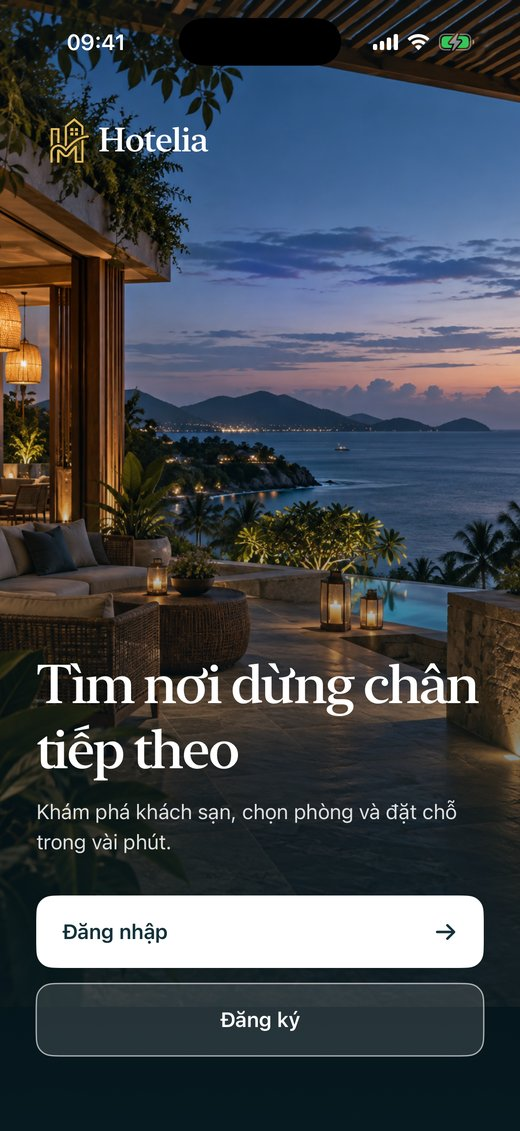
\includegraphics[width=0.3\linewidth]{figures/shots/vi-01-welcome.jpg}}\hfill
\subcaptionbox{Đăng ký}{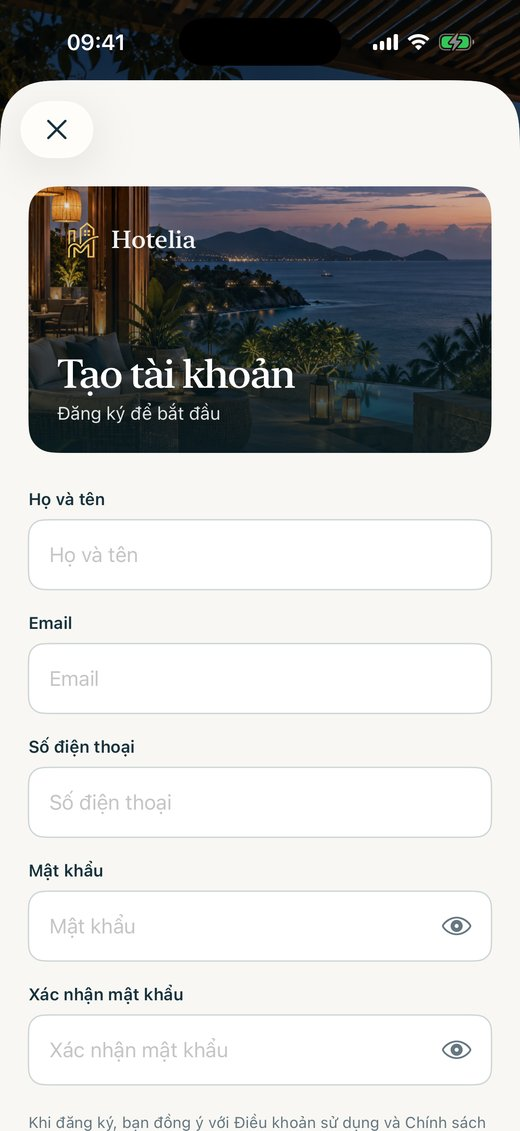
\includegraphics[width=0.3\linewidth]{figures/shots/vi-02-register.jpg}}\hfill
\subcaptionbox{Đăng nhập}{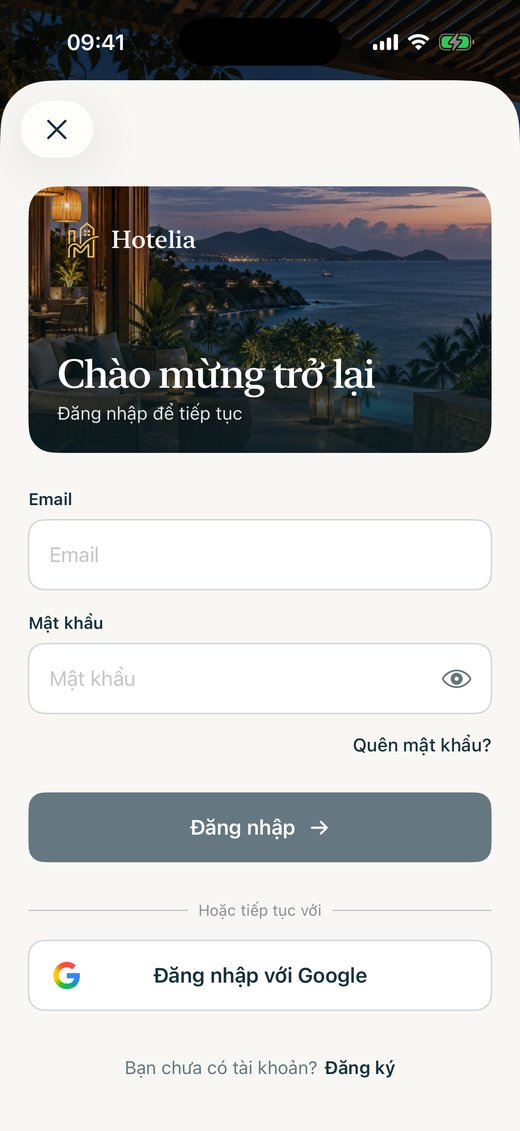
\includegraphics[width=0.3\linewidth]{figures/shots/vi-03-login.jpg}}
\caption{Màn hình chào mừng, đăng ký và đăng nhập}\label{fig:scr-auth}
\end{figure}

\paragraph{Khám phá và gợi ý.} \Cref{fig:scr-explore} là màn Khám phá. Phần đầu có ô tìm điểm đến, bộ chọn ngày, số khách và bộ lọc; tiếp theo là băng chuyền điểm đến và thẻ thời tiết. Cuộn xuống là hàng ``Đề xuất cho bạn''. Với tài khoản đã có lịch sử đặt phòng, dòng mô tả là ``Dựa trên khách sạn bạn đã xem và booking đã xác nhận''. Phần ``Xếp hạng tham khảo'' phân biệt khách sạn có điểm từ đánh giá đã xác minh (nhãn ``Điểm'') với khách sạn chỉ có điểm biên tập (nhãn ``Điểm Hotelia'').

\begin{figure}[H]
\centering
\subcaptionbox{Khám phá, thời tiết}{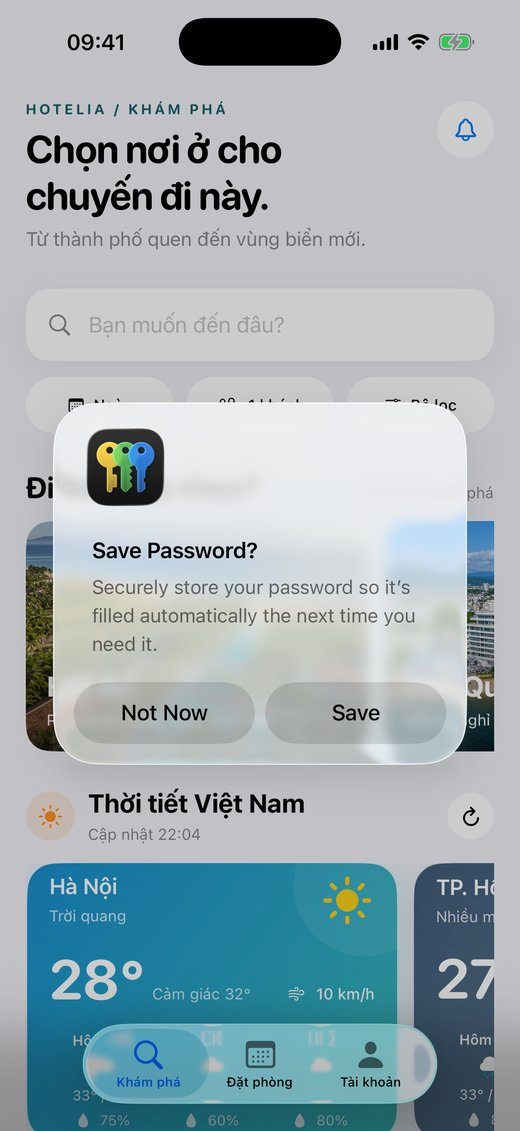
\includegraphics[width=0.3\linewidth]{figures/shots/vi-04-explore.jpg}}\hfill
\subcaptionbox{Đề xuất cho bạn}{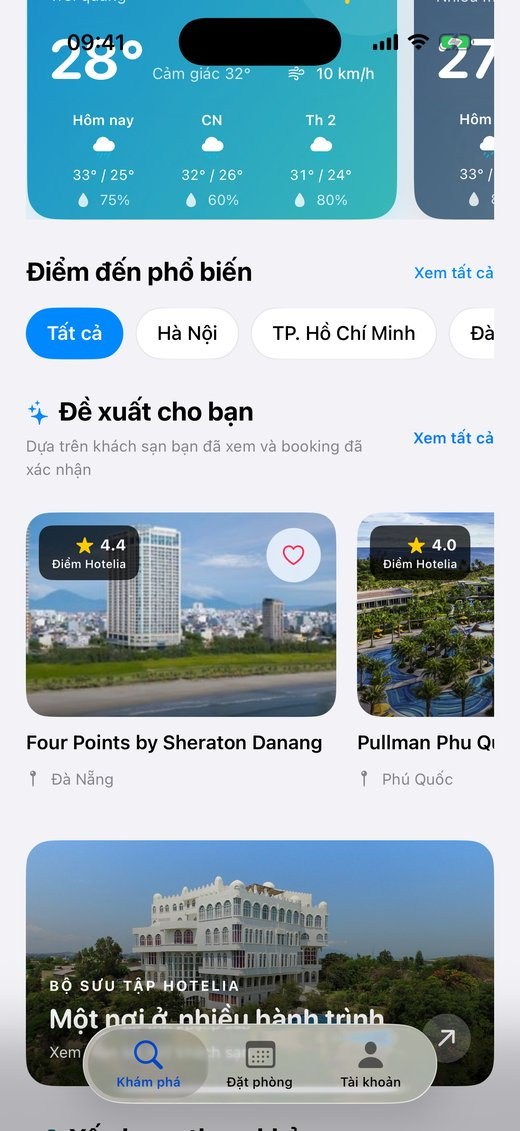
\includegraphics[width=0.3\linewidth]{figures/shots/vi-05-recommend.jpg}}\hfill
\subcaptionbox{Xếp hạng tham khảo}{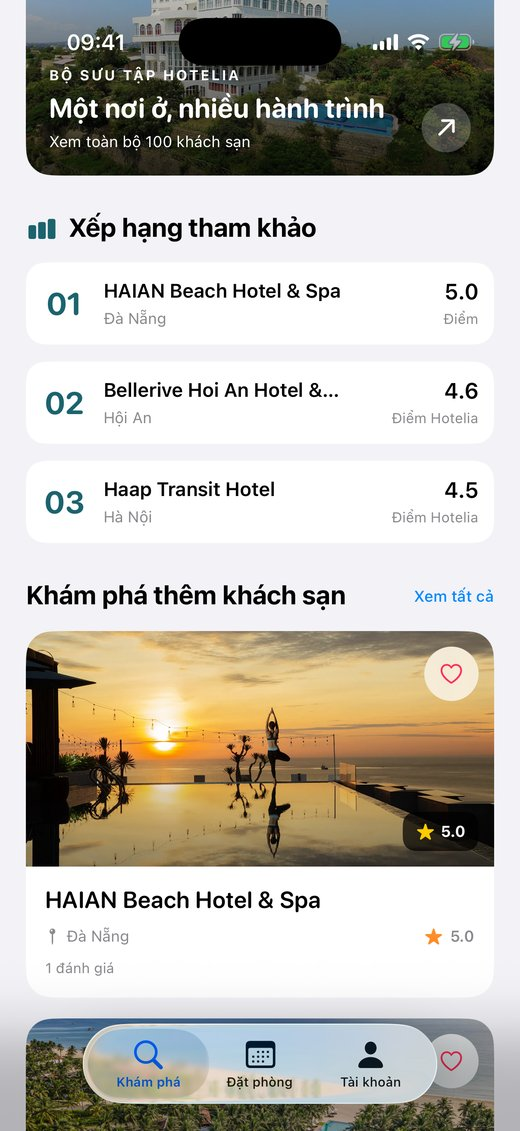
\includegraphics[width=0.3\linewidth]{figures/shots/vi-08-ranking.jpg}}
\caption{Màn Khám phá, thẻ thời tiết và hàng gợi ý cá nhân hóa}\label{fig:scr-explore}
\end{figure}

\paragraph{Chi tiết khách sạn.} \Cref{fig:scr-detail} gồm ảnh, hạng sao, trạng thái ``Đang nhận đặt phòng'', địa chỉ, mô tả, tiện ích, đánh giá và chính sách giờ nhận/trả phòng. Đánh giá đã xác minh (có ngày và phản hồi của khách sạn) được tách khỏi mục ``Nhận xét Hotelia'', mục này kèm dòng chú thích rằng đây không phải đánh giá của khách đã lưu trú.

\begin{figure}[H]
\centering
\subcaptionbox{Thông tin khách sạn}{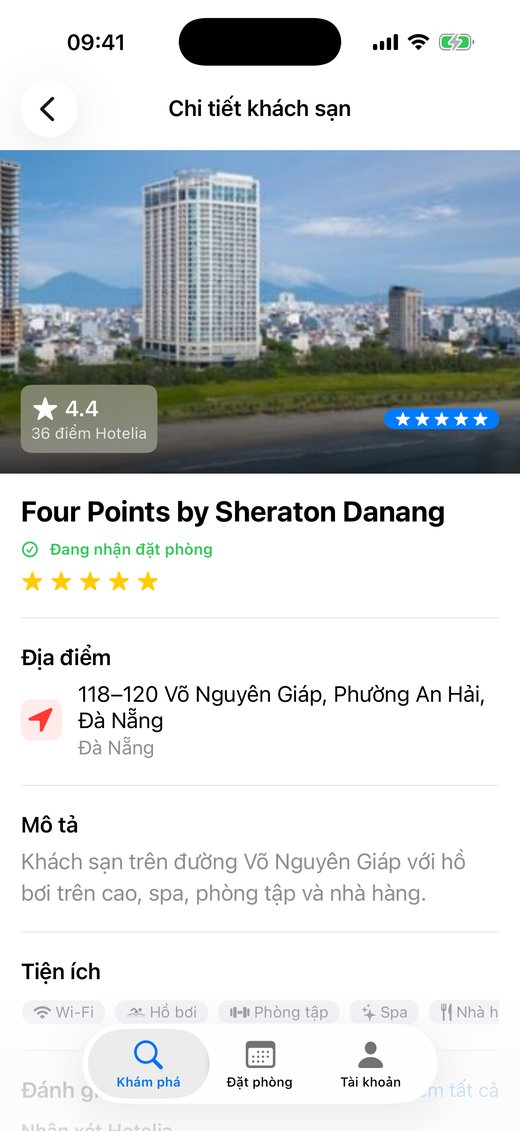
\includegraphics[width=0.3\linewidth]{figures/shots/vi-06-detail.jpg}}\hfill
\subcaptionbox{Đánh giá và phản hồi}{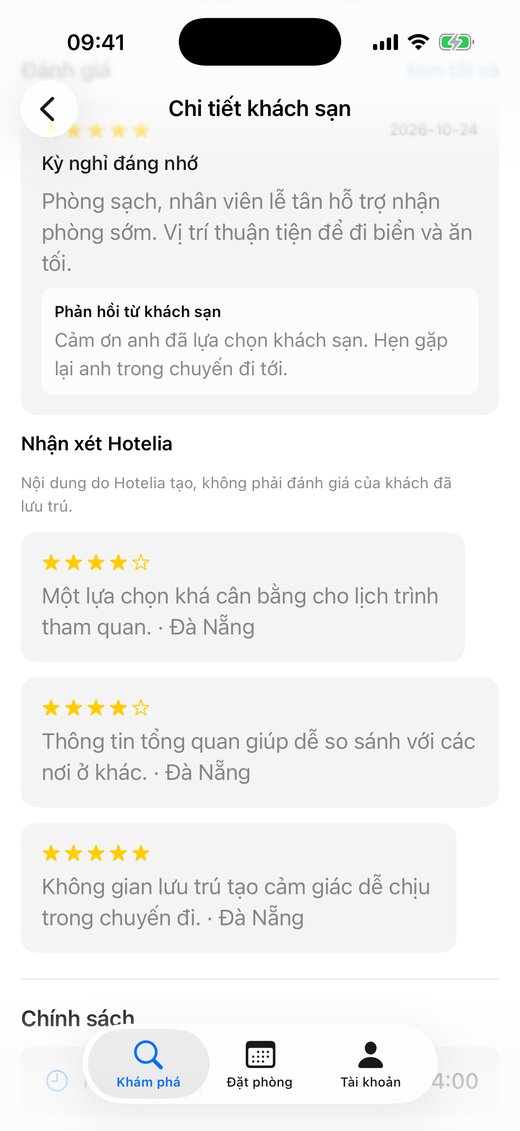
\includegraphics[width=0.3\linewidth]{figures/shots/vi-09-reviews.jpg}}\hfill
\subcaptionbox{Chính sách, đặt phòng}{
\includegraphics[width=0.3\linewidth]{figures/shots/vi-07-detail-policy.jpg}}
\caption{Màn chi tiết khách sạn}\label{fig:scr-detail}
\end{figure}

\paragraph{Chọn phòng và đặt phòng.} \Cref{fig:scr-booking} là màn đặt phòng. Mỗi loại phòng hiển thị ảnh, sức chứa, tiện nghi, giá mỗi đêm và trạng thái chọn. Hai bộ chọn ngày nhận và ngày trả được xếp dọc; cách bố trí này sửa lỗi tràn ngang do chuỗi ngày tiếng Việt dài (\cref{sec:test-ui}). Phần cuối hiển thị tạm tính và các ghi chú về thời gian giữ phòng, chính sách hủy.

\begin{figure}[H]
\centering
\subcaptionbox{Chọn loại phòng}{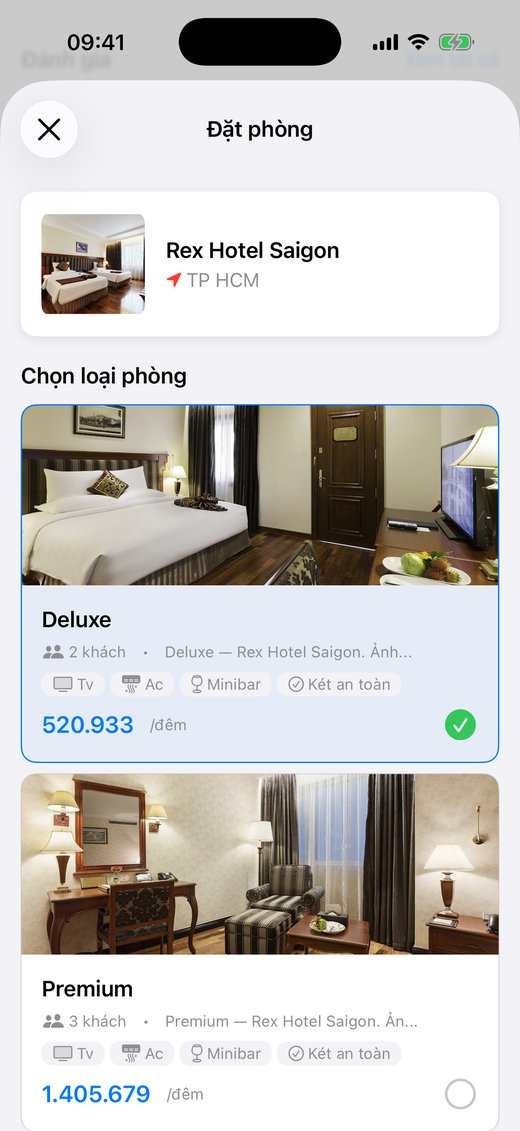
\includegraphics[width=0.3\linewidth]{figures/shots/vi-10-rooms.jpg}}\hfill
\subcaptionbox{Ngày, số khách}{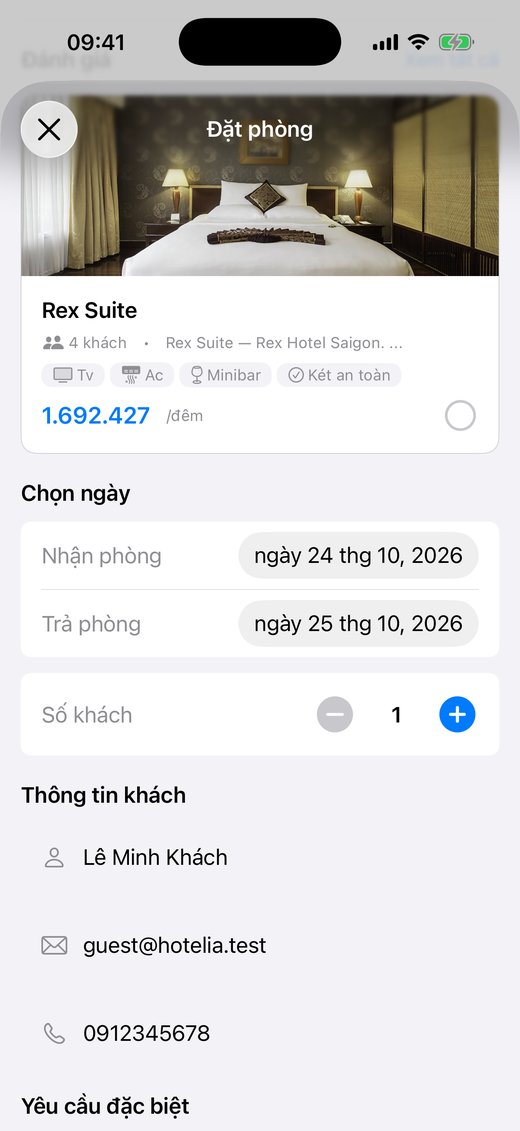
\includegraphics[width=0.3\linewidth]{figures/shots/vi-11-dates.jpg}}\hfill
\subcaptionbox{Đã giữ phòng}{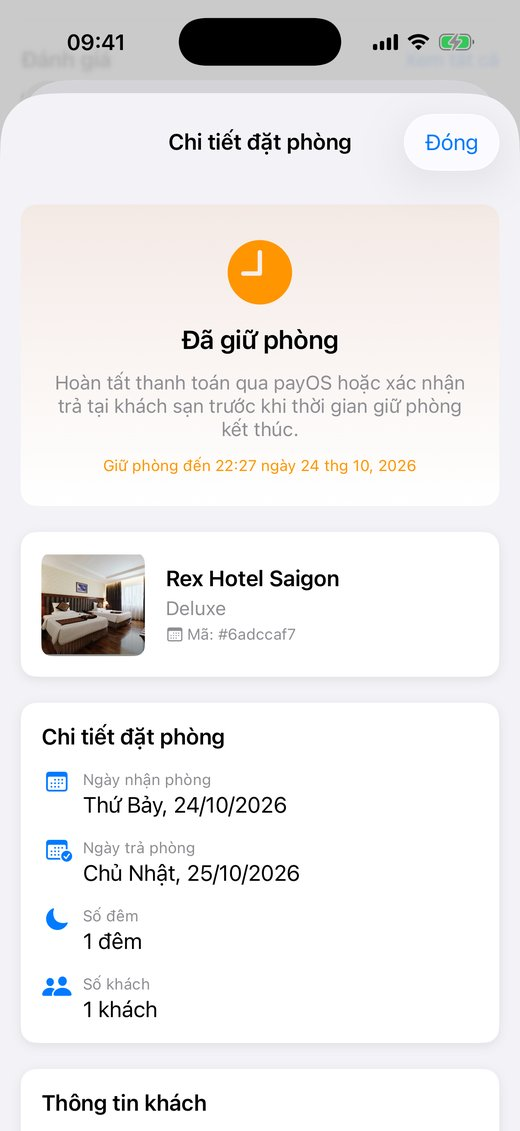
\includegraphics[width=0.3\linewidth]{figures/shots/vi-12-hold.jpg}}
\caption{Luồng chọn phòng, chọn ngày và giữ phòng}\label{fig:scr-booking}
\end{figure}

\paragraph{Thanh toán.} \Cref{fig:scr-payment} là phần thanh toán của chi tiết đặt phòng. Ảnh (b) cho thấy hành vi khi máy chủ chưa cấu hình khóa payOS: ứng dụng hiển thị ``Kênh thanh toán payOS chưa được cấu hình'' do máy chủ trả mã 503. Hệ thống không tạo đơn thanh toán nào. Ảnh (c) là lịch sử sau khi khách chọn ``Thanh toán tại khách sạn'': đặt phòng chuyển sang ``Đã xác nhận''.

\begin{figure}[H]
\centering
\subcaptionbox{Phương thức thanh toán}{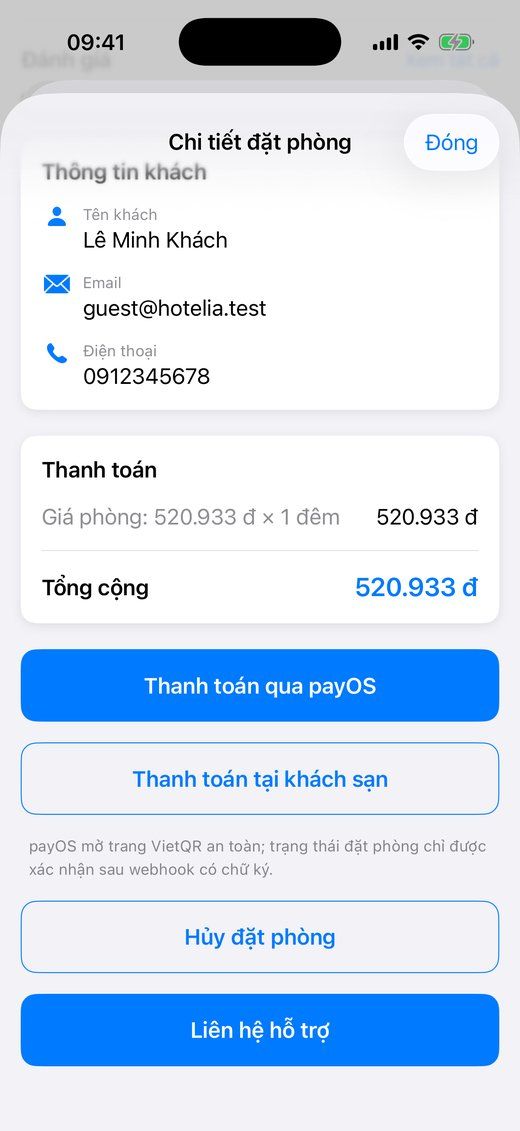
\includegraphics[width=0.3\linewidth]{figures/shots/vi-13-payment.jpg}}\hfill
\subcaptionbox{payOS chưa cấu hình}{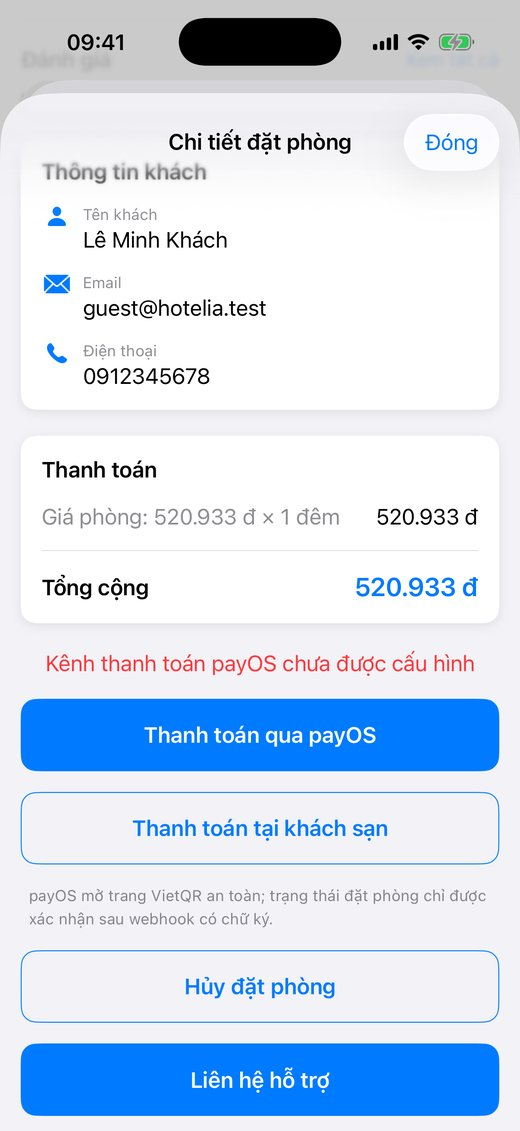
\includegraphics[width=0.3\linewidth]{figures/shots/vi-14-payos-unconfigured.jpg}}\hfill
\subcaptionbox{Đã xác nhận}{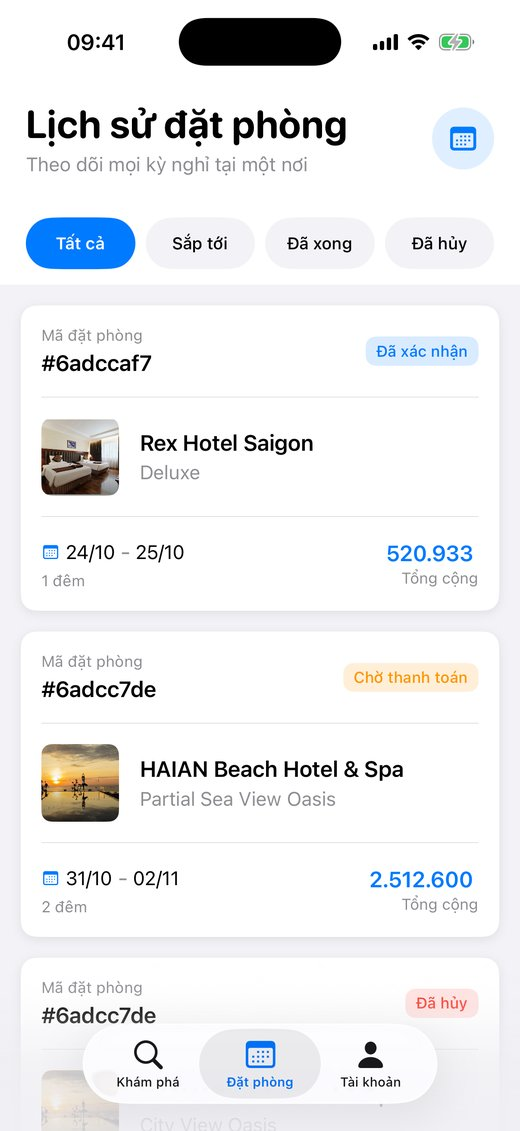
\includegraphics[width=0.3\linewidth]{figures/shots/vi-15-history.jpg}}
\caption{Thanh toán và xác nhận đặt phòng}\label{fig:scr-payment}
\end{figure}

\paragraph{Lịch sử đặt phòng và tài khoản.} \Cref{fig:scr-account} gồm lịch sử với nhiều trạng thái (đã nhận phòng, đã trả phòng), màn tài khoản và lựa chọn ngôn ngữ. Màn tài khoản là lối vào cho khách sạn đã lưu, đăng ký làm đối tác, hồ sơ, thông báo, bảo mật, ngôn ngữ, trợ giúp và màn quản lý dành cho chủ khách sạn/quản trị viên.

\begin{figure}[H]
\centering
\subcaptionbox{Trạng thái đặt phòng}{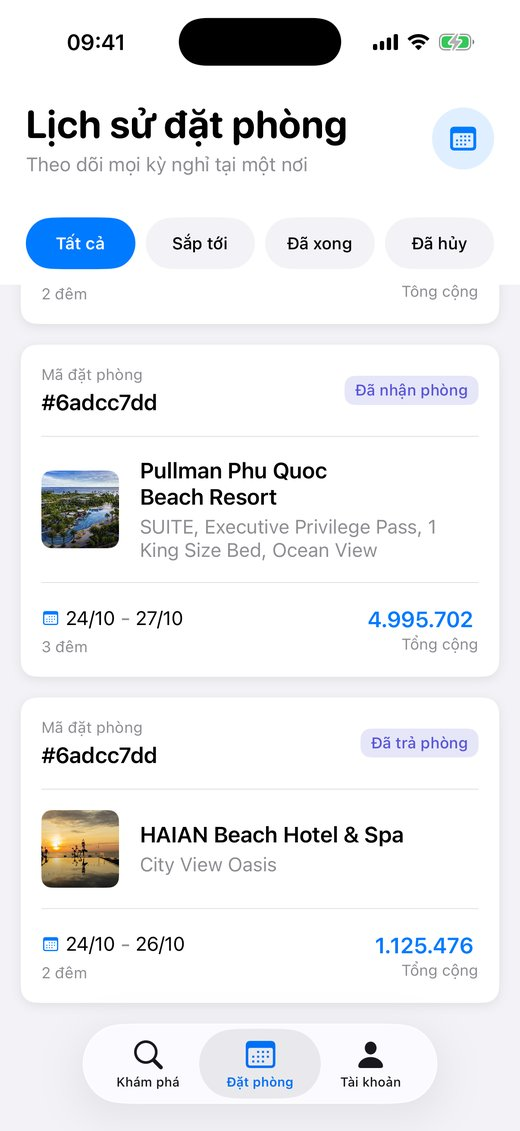
\includegraphics[width=0.3\linewidth]{figures/shots/vi-16-history-states.jpg}}\hfill
\subcaptionbox{Tài khoản}{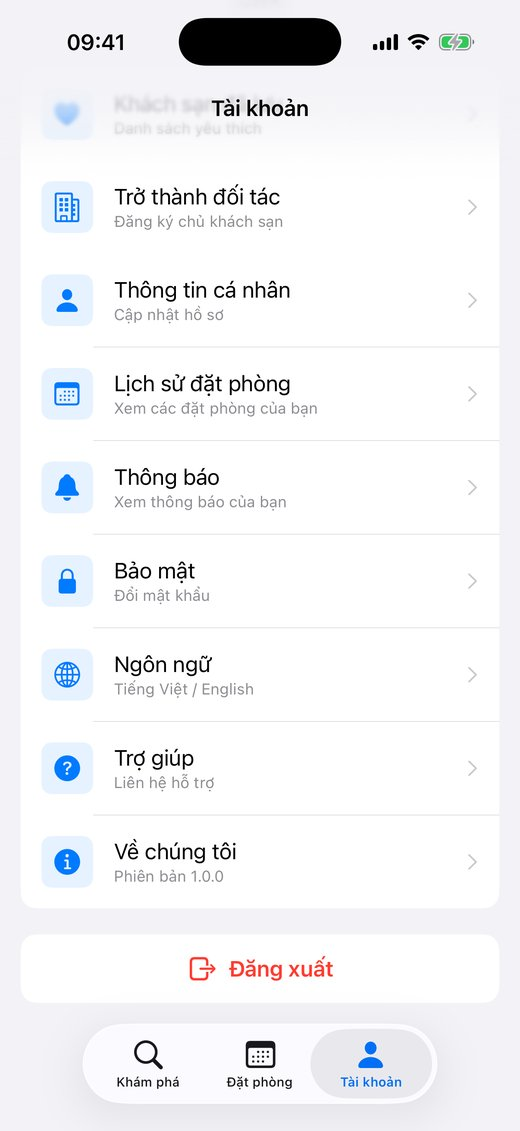
\includegraphics[width=0.3\linewidth]{figures/shots/vi-18-profile-menu.jpg}}\hfill
\subcaptionbox{Ngôn ngữ}{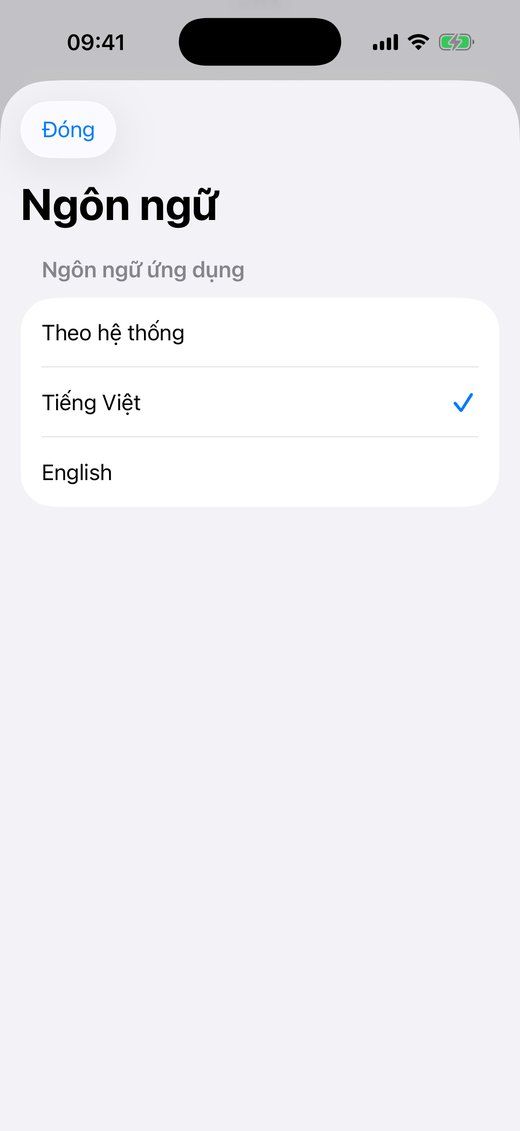
\includegraphics[width=0.3\linewidth]{figures/shots/vi-19-language.jpg}}
\caption{Lịch sử đặt phòng, tài khoản và chọn ngôn ngữ}\label{fig:scr-account}
\end{figure}

\paragraph{Giao diện tiếng Anh.} \Cref{fig:scr-english} là cùng các màn hình khi chọn tiếng Anh. Định dạng số đổi theo ngôn ngữ (``520,933'' thay vì ``520.933''). Nhãn trạng thái được dịch, kể cả ``Expired'' của đặt phòng đã hết hạn giữ.

\begin{figure}[H]
\centering
\subcaptionbox{Welcome}{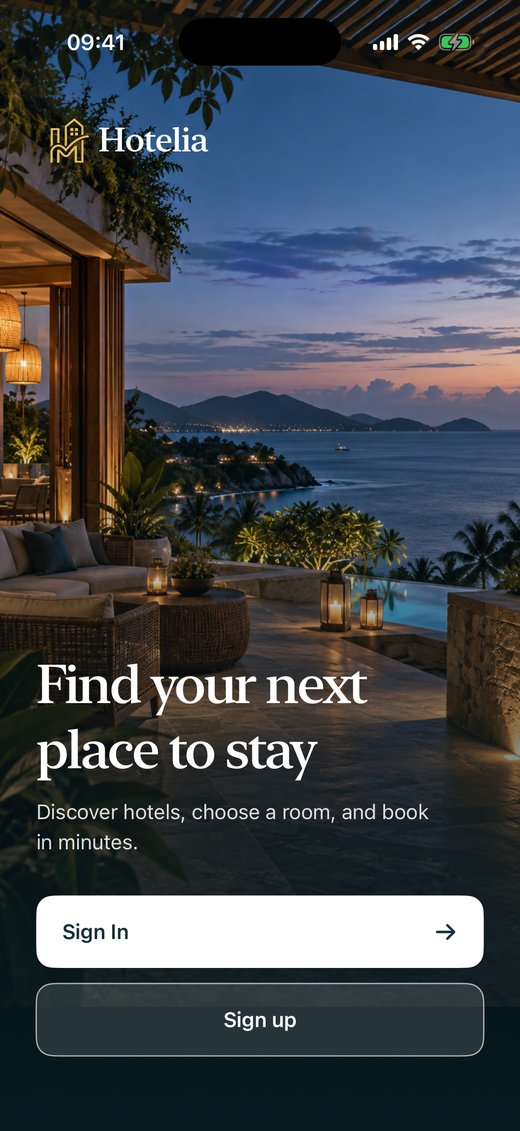
\includegraphics[width=0.3\linewidth]{figures/shots/en-01-welcome.jpg}}\hfill
\subcaptionbox{Explore}{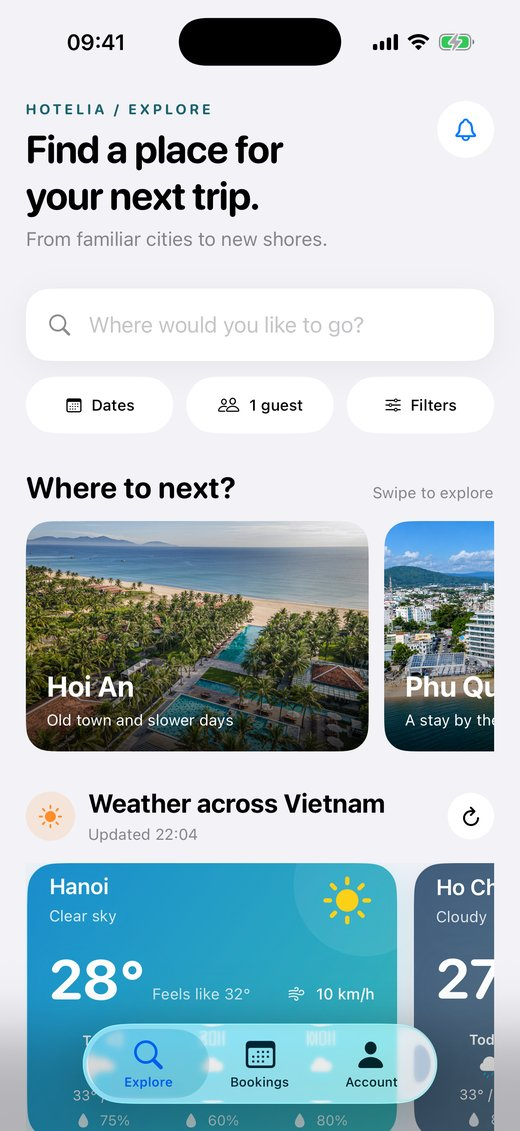
\includegraphics[width=0.3\linewidth]{figures/shots/en-04-explore.jpg}}\hfill
\subcaptionbox{Booking history}{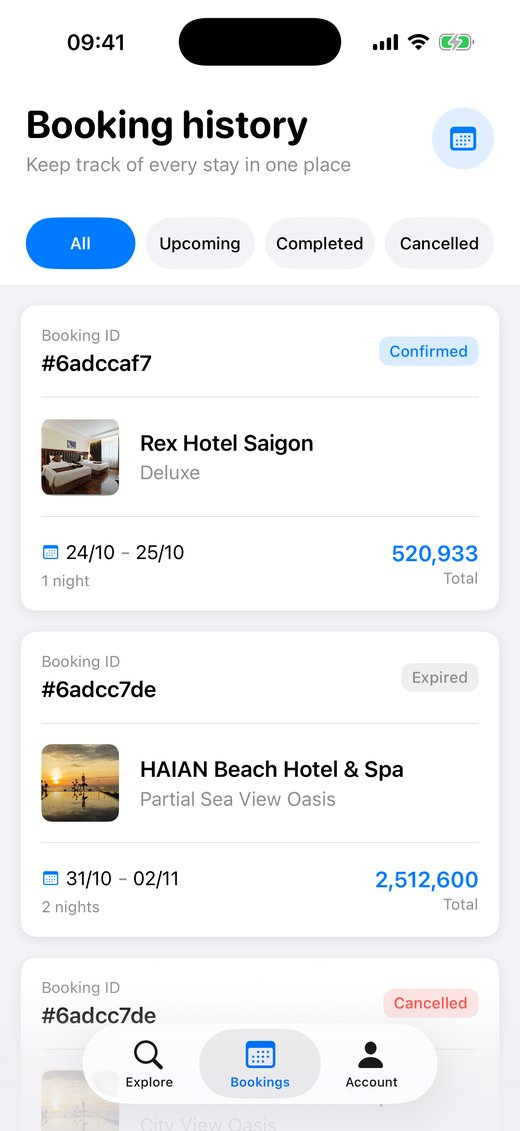
\includegraphics[width=0.3\linewidth]{figures/shots/en-05-history.jpg}}
\caption{Giao diện tiếng Anh của ứng dụng}\label{fig:scr-english}
\end{figure}

\section{Cài đặt máy chủ NestJS}\label{sec:impl-backend}

\subsection{Khởi động và cấu hình}

Tệp \code{main.ts} cấu hình các thành phần toàn cục:
\begin{itemize}
\item CORS: ở môi trường vận hành chỉ chấp nhận các nguồn khai báo trong \code{CORS\_ORIGINS}; ở môi trường phát triển chấp nhận thêm các cổng localhost của Vite.
\item Tiền tố \code{/api}, phiên bản URI mặc định \code{v1}.
\item \code{ValidationPipe} với \code{whitelist}, \code{forbidNonWhitelisted}, \code{transform}.
\item \code{HttpExceptionFilter}; thư mục ảnh tĩnh \code{/media/} không liệt kê thư mục và từ chối tệp ẩn.
\item Tài liệu Swagger, chỉ bật ở môi trường phát triển.
\end{itemize}
Hàm \code{validateEnvironment} kiểm tra cấu hình ngay khi khởi động. Máy chủ từ chối chạy ở môi trường vận hành nếu \code{JWT\_SECRET} ngắn hơn 32 ký tự hoặc trông như giá trị mẫu, nếu thiếu \code{CORS\_ORIGINS}, hoặc nếu chỉ có một phần trong ba khóa payOS. Bốn ca kiểm thử trong \code{env.validation.spec.ts} kiểm chứng các điều kiện này.

\subsection{Xác thực và phân quyền}\label{sec:impl-auth}

\Cref{lst:tokens} là hàm phát hành token. Trong quá trình viết báo cáo, việc đối chiếu với RFC 8725 \cite{rfc8725} cho thấy phiên bản cũ ký access token và refresh token bằng cùng khóa và cùng nội dung. Hệ quả là một refresh token có hạn 7 ngày cũng được \code{JwtStrategy} chấp nhận như access token. Bản sửa thêm claim \code{typ} vào mỗi token. \code{JwtStrategy} từ chối token có \code{typ = refresh} (\cref{lst:jwt}); điểm cuối làm mới từ chối token có \code{typ = access}. Token phát hành trước bản sửa không có \code{typ} và vẫn được chấp nhận cho tới khi hết hạn, để người dùng đang đăng nhập không bị đăng xuất đột ngột. Bốn ca kiểm thử mới kiểm chứng hành vi này.

Khi bổ sung chức năng thu hồi phiên lúc đăng xuất, báo cáo phát hiện thêm một lỗi trong cách lưu refresh token. Phiên bản cũ lưu \code{bcrypt(refreshToken)}, nhưng bcrypt chỉ đọc 72 byte đầu của đầu vào. Mọi refresh token của cùng một người dùng có chung 72 byte đầu (phần header và claim \code{sub}), nên token cũ vẫn khớp với bản băm của token mới và việc xoay vòng không vô hiệu hóa được token cũ. Ngoài ra, hai token phát hành trong cùng một giây có nội dung giống hệt nhau. Bản sửa gồm ba phần: (i) lưu bản băm SHA-256 của toàn bộ token và so sánh bằng \code{timingSafeEqual}; vì refresh token là chuỗi ngẫu nhiên dài do máy chủ ký nên không cần hàm băm chậm như với mật khẩu; (ii) thêm claim \code{jti} ngẫu nhiên vào mỗi refresh token (\cref{lst:tokens}); (iii) điểm cuối \code{POST /auth/logout} nhận chính refresh token cần thu hồi thay vì access token, nên đăng xuất vẫn có hiệu lực khi access token đã hết hạn. Bản băm bcrypt cũ vẫn được chấp nhận ở lần làm mới kế tiếp rồi được thay bằng SHA-256, để người dùng đang đăng nhập không bị đăng xuất khi triển khai. Ứng dụng iOS và bảng điều khiển gọi điểm cuối này ở nền khi người dùng đăng xuất.

\lstinputlisting[language=TypeScript, firstnumber=121, caption={Phát hành access token và refresh token có phân loại (\code{auth.service.ts})}, label={lst:tokens}]{code/auth-generate-tokens.ts}

\lstinputlisting[language=TypeScript, firstnumber=20, caption={Kiểm tra token ở mỗi yêu cầu (\code{jwt.strategy.ts})}, label={lst:jwt}]{code/jwt-validate.ts}

\code{JwtStrategy} đọc lại người dùng ở mỗi yêu cầu. Nhờ đó ba thay đổi có hiệu lực ngay: tài khoản bị khóa (\code{isActive = false}), mật khẩu vừa đổi (\code{tokenVersion} tăng), và vai trò vừa được nâng lên OWNER. Đổi lại, mỗi yêu cầu tốn thêm một truy vấn theo khóa chính. \code{RolesGuard} so khớp vai trò với danh sách khai báo bằng decorator \code{@Roles}. Kiểm tra quyền sở hữu được viết tường minh trong từng dịch vụ, ví dụ \code{String(hotel.ownerId) !== ownerId}.

\subsection{Máy trạng thái và giao dịch đặt phòng}\label{sec:impl-booking}

\Cref{lst:states} là bảng chuyển trạng thái được khai báo tường minh. \Cref{lst:rules} là các hàm thuần túy cài đặt quy tắc chiếm tồn kho, hết hạn giữ và đếm phòng trống theo đêm (\cref{eq:free-rooms}). Do là hàm thuần túy, chúng được kiểm thử trực tiếp mà không cần cơ sở dữ liệu.

\lstinputlisting[language=TypeScript, firstnumber=18, caption={Bảng chuyển trạng thái đặt phòng (\code{booking-state.service.ts})}, label={lst:states}]{code/booking-states.ts}

\lstinputlisting[language=TypeScript, firstnumber=3, caption={Quy tắc ngày, chiếm tồn kho và đếm phòng trống (\code{booking-rules.ts})}, label={lst:rules}]{code/booking-rules.ts}

\Cref{lst:create} là phần giao dịch của \code{BookingsService.create}. Ba chi tiết quan trọng là: (i) lệnh \code{findOneAndUpdate} tăng \code{inventoryVersion} nằm \emph{trước} truy vấn đếm, nên hai giao dịch đồng thời xung đột ngay tại tài liệu loại phòng; (ii) giá được lấy từ loại phòng trong giao dịch, không lấy từ yêu cầu; (iii) khối \code{catch} tra lại theo khóa lũy đẳng, vì khi hai yêu cầu cùng khóa chạy đồng thời, yêu cầu thua có thể gặp lỗi trùng chỉ mục duy nhất trong khi đặt phòng đã tồn tại.

\lstinputlisting[language=TypeScript, firstnumber=39, caption={Giao dịch tạo đặt phòng (\code{bookings.service.ts})}, label={lst:create}]{code/bookings-create-tx.ts}

Mọi thay đổi trạng thái sau đó đi qua hàm \code{transition}: cập nhật có điều kiện \code{\{\_id, status: trạng thái cũ\}}. Nếu không có tài liệu nào khớp, hàm đọc lại đặt phòng. Nếu trạng thái hiện tại đã là trạng thái đích, hàm trả về thành công; nếu không, hàm báo ``Booking đã thay đổi. Vui lòng tải lại''.

\subsection{Thanh toán và webhook}\label{sec:impl-payment}

\code{PayOSClient} bao thư viện \code{@payos/node} \cite{payosnode} với thời gian chờ 10 giây, tối đa 2 lần thử lại. Lỗi được chuyển thành mã HTTP có nghĩa: hết thời gian chờ thành 502 ``payOS không phản hồi trong thời gian cho phép'', thiếu cấu hình thành 503. \Cref{lst:verify} là hàm xác minh webhook. Thư viện tính lại HMAC-SHA256 bằng \code{checksumKey}; chữ ký sai làm webhook bị từ chối với mã 400.

\lstinputlisting[language=TypeScript, firstnumber=101, caption={Xác minh chữ ký webhook payOS (\code{payos.client.ts})}, label={lst:verify}]{code/payos-verify.ts}

\Cref{lst:webhook} là phần xử lý webhook đã xác minh. Webhook mẫu mà payOS gửi khi đăng ký địa chỉ webhook không khớp đơn nào và được trả lời ``đã xác minh'' mà không thay đổi dữ liệu. Webhook thật được xử lý trong một giao dịch: bỏ qua nếu thanh toán đã COMPLETED (lũy đẳng), dừng nếu số tiền lệch. Phần tiếp theo của giao dịch (không in ở đây) chuyển thanh toán sang COMPLETED; nếu đặt phòng còn PENDING\_PAYMENT thì chuyển sang CONFIRMED, hoặc sang CANCEL\_REQUESTED với lý do \code{PAYMENT\_AFTER\_HOLD\_EXPIRED} khi giữ phòng đã hết hạn; cuối cùng ghi thông báo cho khách.

\lstinputlisting[language=TypeScript, firstnumber=174, caption={Xử lý webhook payOS trong giao dịch (\code{payments.service.ts})}, label={lst:webhook}]{code/payments-webhook.ts}

Việc hoàn tiền chưa được cài đặt: \code{PaymentsService.refund} luôn trả 503 kèm thông điệp cần đối soát thủ công. Báo cáo ghi nhận đây là giới hạn (\cref{sec:limitations}).

\subsection{Nhật ký thao tác và giới hạn tần suất}

\code{AuditInterceptor} được đăng ký toàn cục. Sau mỗi yêu cầu POST, PUT, PATCH, DELETE thành công của người dùng đã đăng nhập (trừ nhóm \code{/auth/}), interceptor ghi \code{actorId}, \code{role}, \code{method}, \code{path} vào \code{audit\_logs}. Nội dung yêu cầu không được lưu, nên mật khẩu hay thông tin cá nhân không lọt vào nhật ký. Lỗi ghi nhật ký chỉ được cảnh báo, không làm hỏng yêu cầu chính. \code{ThrottlerGuard} giới hạn 100 yêu cầu mỗi 60 giây.

\section{Cài đặt bảng điều khiển React}\label{sec:impl-web}

\subsection{Cấu trúc và xác thực}

Bảng điều khiển gồm các thư mục \code{features/owner}, \code{features/admin}, \code{features/auth}, \code{components/ui} (Button, Card, Badge, StatCard, Input), \code{components/layout} (Sidebar, Layout), \code{lib/api/client.ts} và \code{lib/auth/AuthContext.tsx}. Client Axios gắn access token vào mọi yêu cầu. Khi gặp 401, client làm mới token một lần; các yêu cầu đồng thời dùng chung một promise làm mới (\code{refreshInFlight}), tương tự actor ở phía iOS. Thành phần \code{PrivateRoute} kiểm tra vai trò trước khi hiển thị nhánh \code{/owner/*} hoặc \code{/admin/*}.

\subsection{Màn hình chủ khách sạn}

\Cref{fig:web-owner} là các màn hình của chủ khách sạn, chụp ở độ phân giải 1440$\times$900. Bảng điều khiển tổng quan có bốn chỉ số (khách sạn, đã đăng, đặt phòng, đang lưu trú) và biểu đồ giá trị đặt phòng được xác nhận theo tháng. Màn ``Đơn đặt phòng'' liệt kê đặt phòng với nhãn trạng thái và thao tác nhận phòng, trả phòng, xác nhận hủy. Màn ``Đánh giá'' cho phép phản hồi đánh giá của khách.

\begin{figure}[H]
\centering
\subcaptionbox{Tổng quan khách sạn\label{fig:web-owner-dash}}{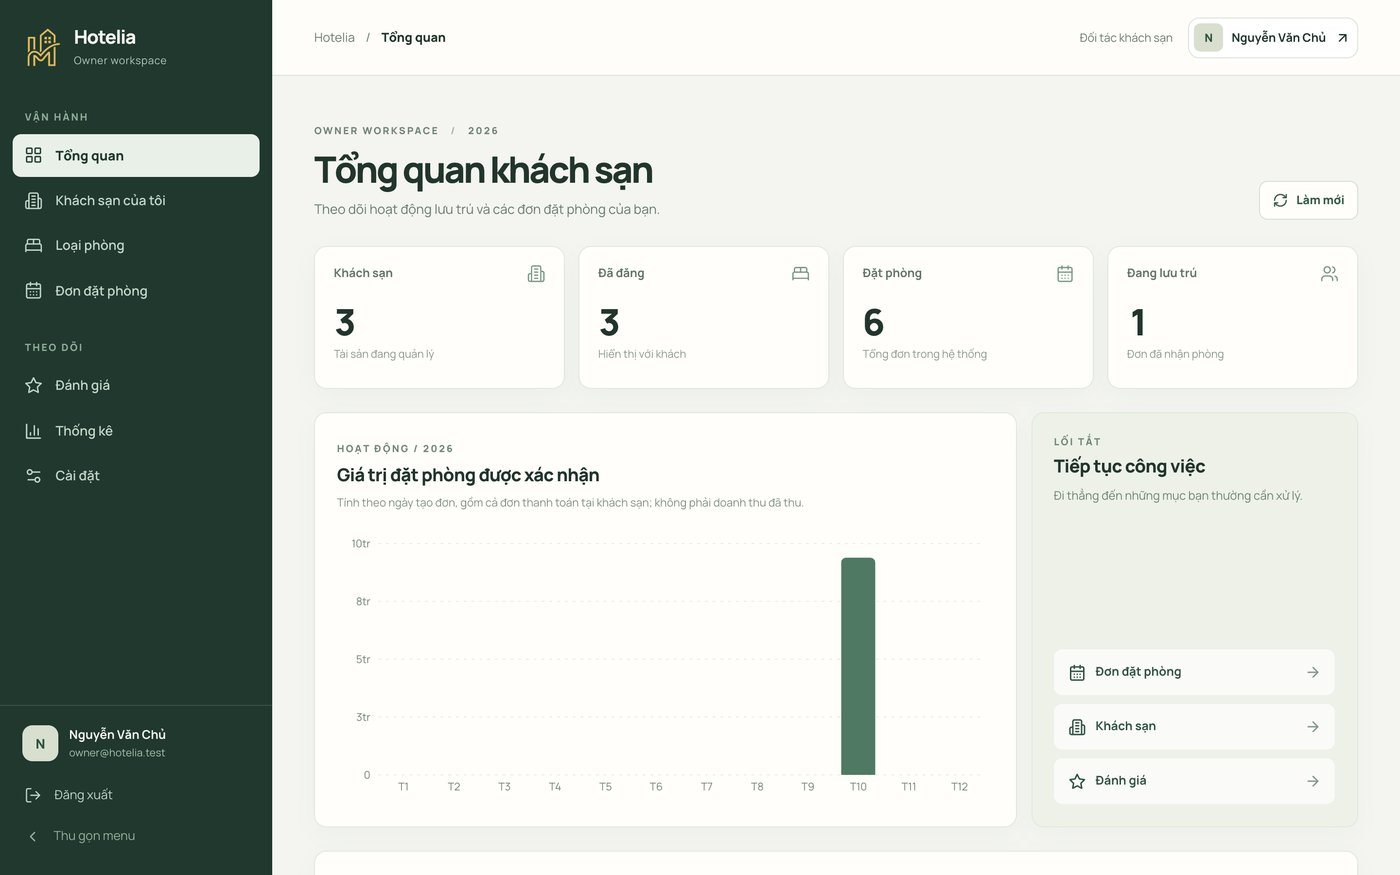
\includegraphics[width=0.49\linewidth]{figures/shots/web-02-owner-dashboard.jpg}}\hfill
\subcaptionbox{Khách sạn của tôi}{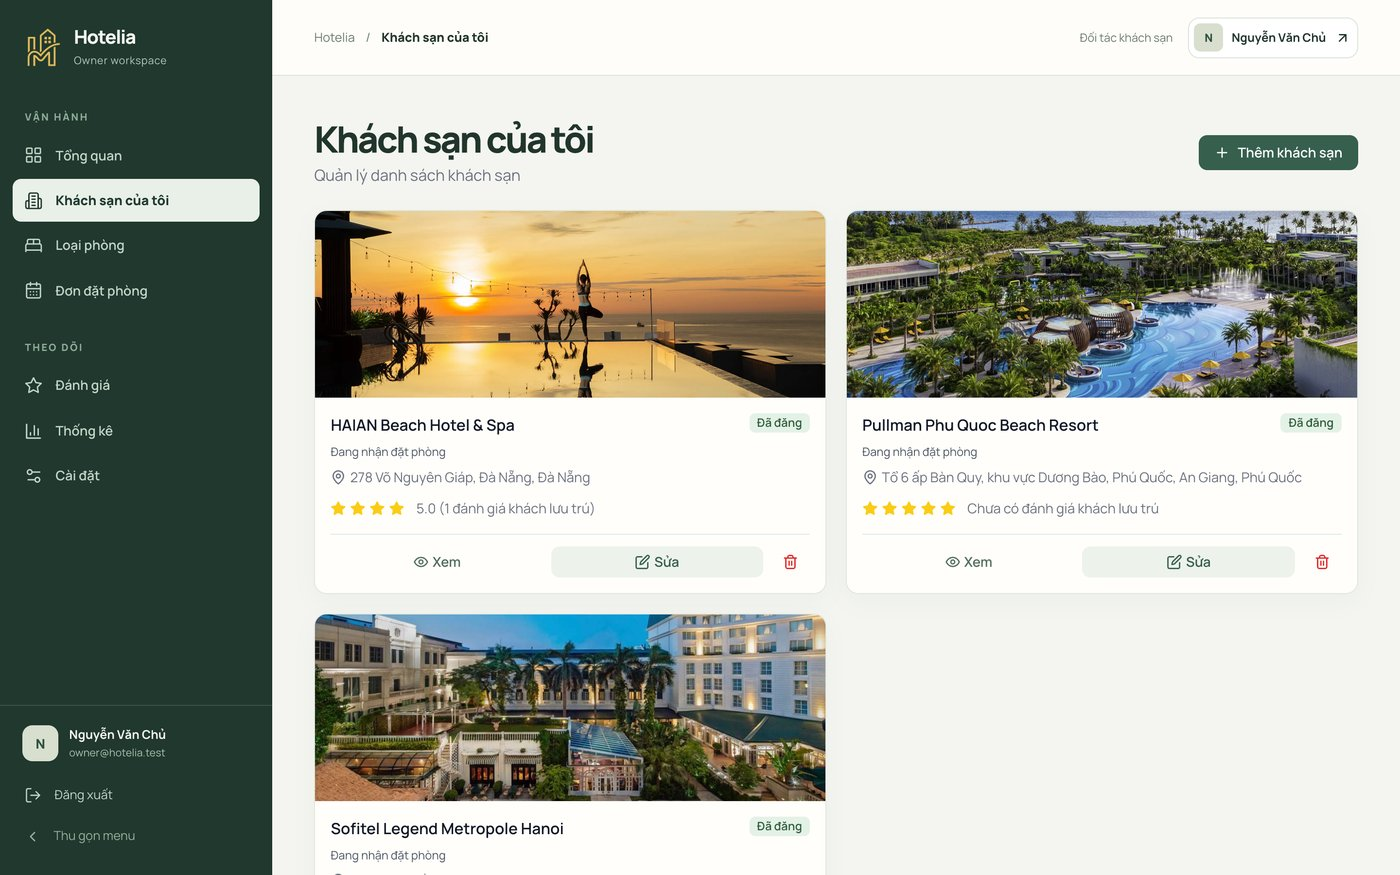
\includegraphics[width=0.49\linewidth]{figures/shots/web-03-owner-hotels.jpg}}\\[6pt]
\subcaptionbox{Đơn đặt phòng}{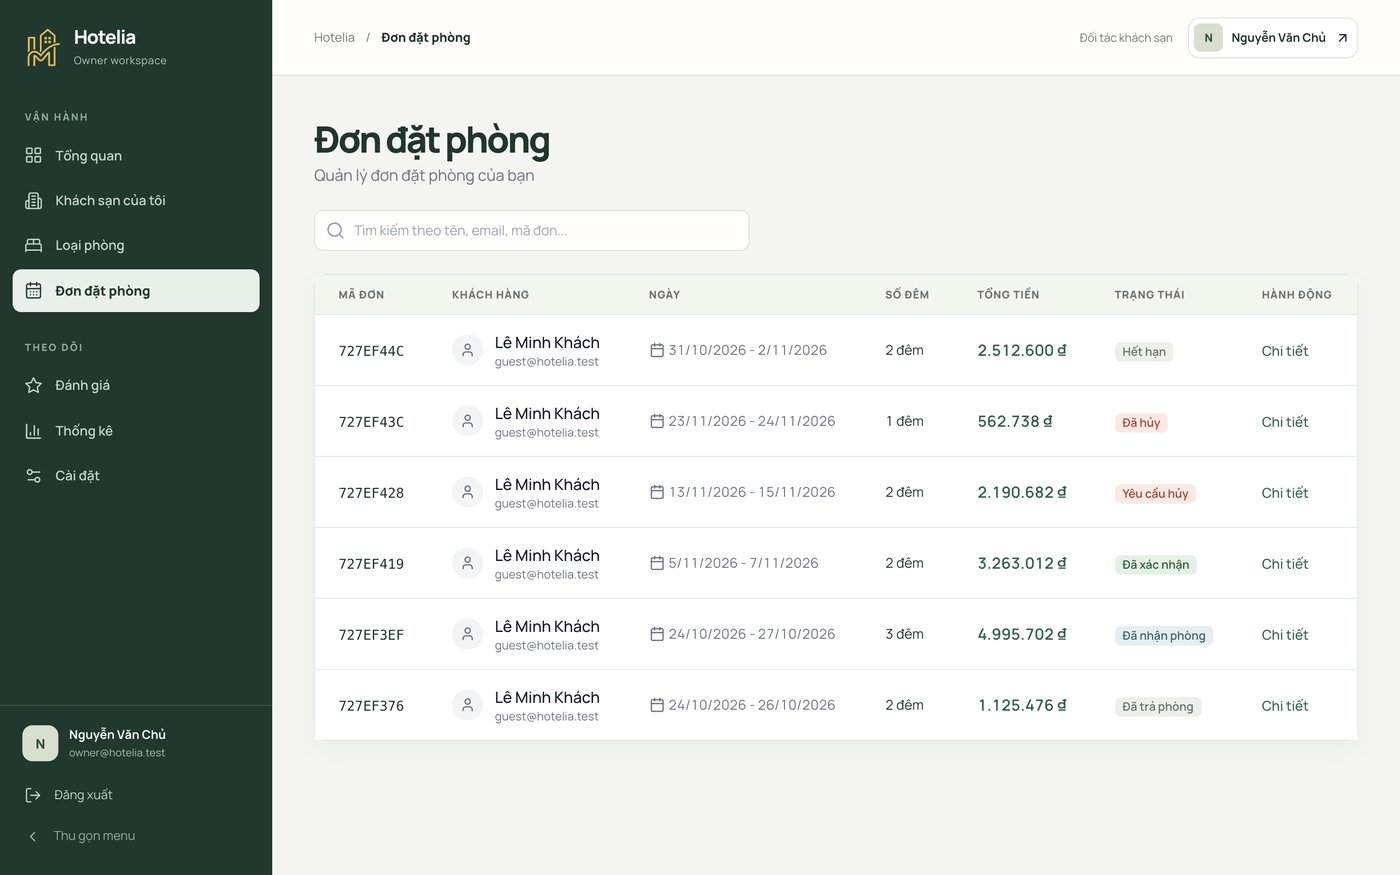
\includegraphics[width=0.49\linewidth]{figures/shots/web-04-owner-bookings.jpg}}\hfill
\subcaptionbox{Đánh giá và phản hồi}{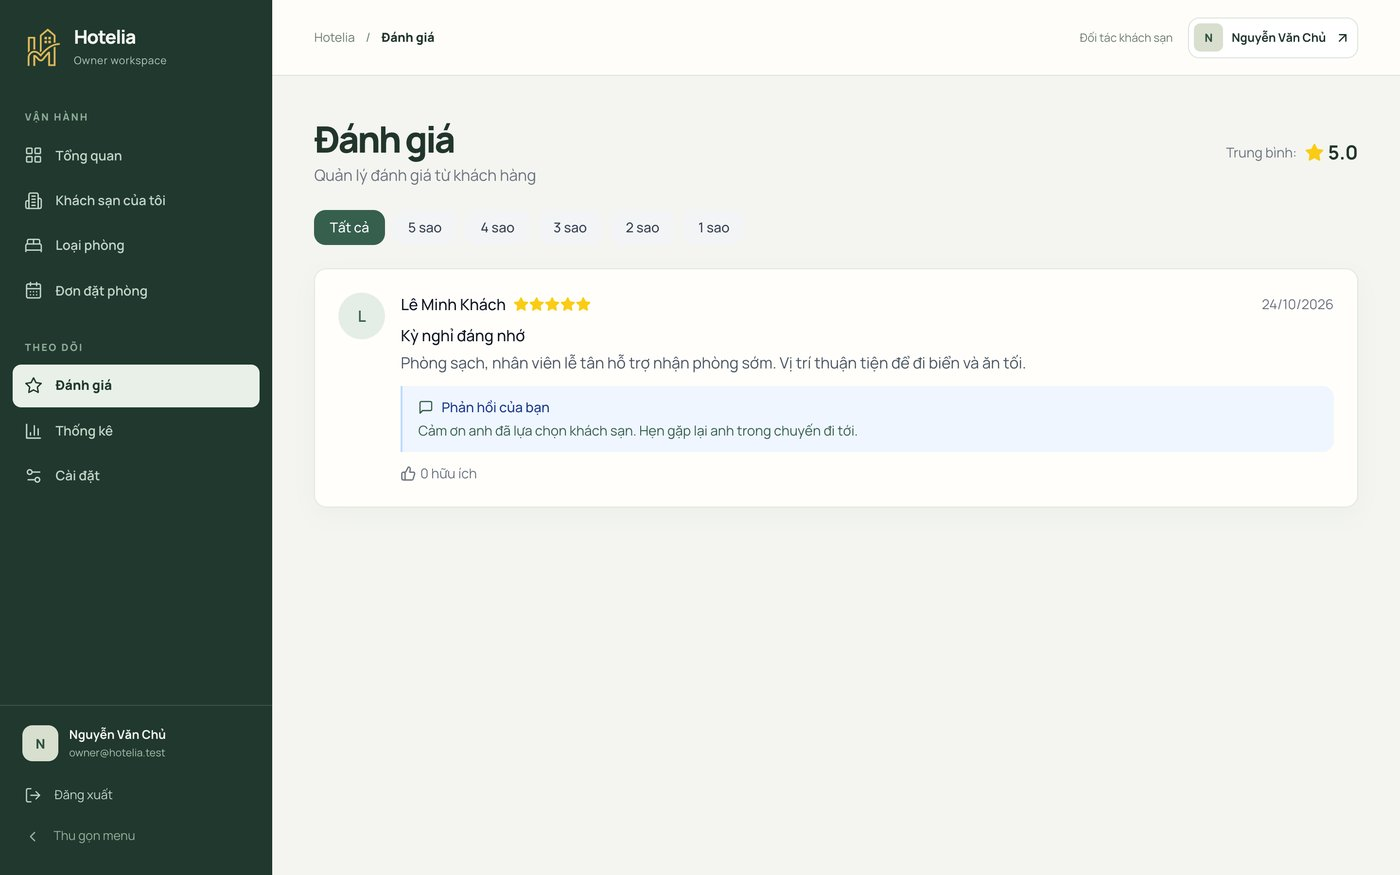
\includegraphics[width=0.49\linewidth]{figures/shots/web-05-owner-reviews.jpg}}
\caption{Bảng điều khiển của chủ khách sạn}\label{fig:web-owner}
\end{figure}

\subsection{Màn hình quản trị viên}

\Cref{fig:web-admin} là các màn hình của quản trị viên. Màn ``Chủ khách sạn'' hiển thị số hồ sơ chờ duyệt, đã duyệt, bị từ chối và nút duyệt/từ chối cho hồ sơ đang chờ. Màn ``Quản lý khách sạn'' có bộ lọc theo trạng thái và cho biết khách sạn nào đang nhận đặt phòng. Màn ``Thanh toán'' ghi rõ rằng giao dịch payOS chỉ được đánh dấu COMPLETED sau khi máy chủ xác thực chữ ký webhook, và đơn trả tại khách sạn không phải giao dịch đã thu tiền. Màn ``Nhật ký thao tác'' hiển thị tối đa 200 thao tác gần nhất.

\begin{figure}[H]
\centering
\subcaptionbox{Tổng quan hệ thống}{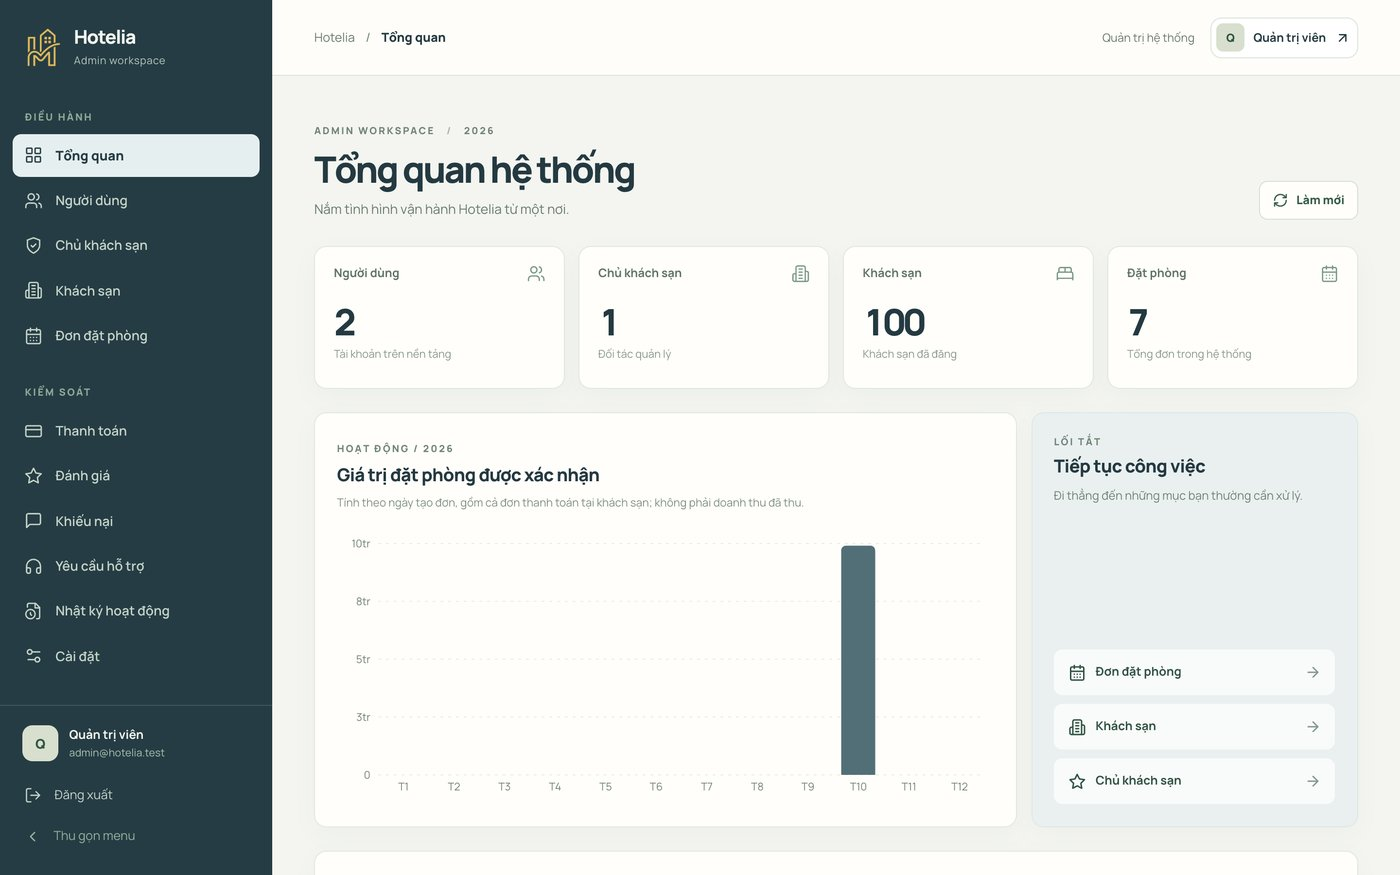
\includegraphics[width=0.49\linewidth]{figures/shots/web-06-admin-dashboard.jpg}}\hfill
\subcaptionbox{Duyệt chủ khách sạn}{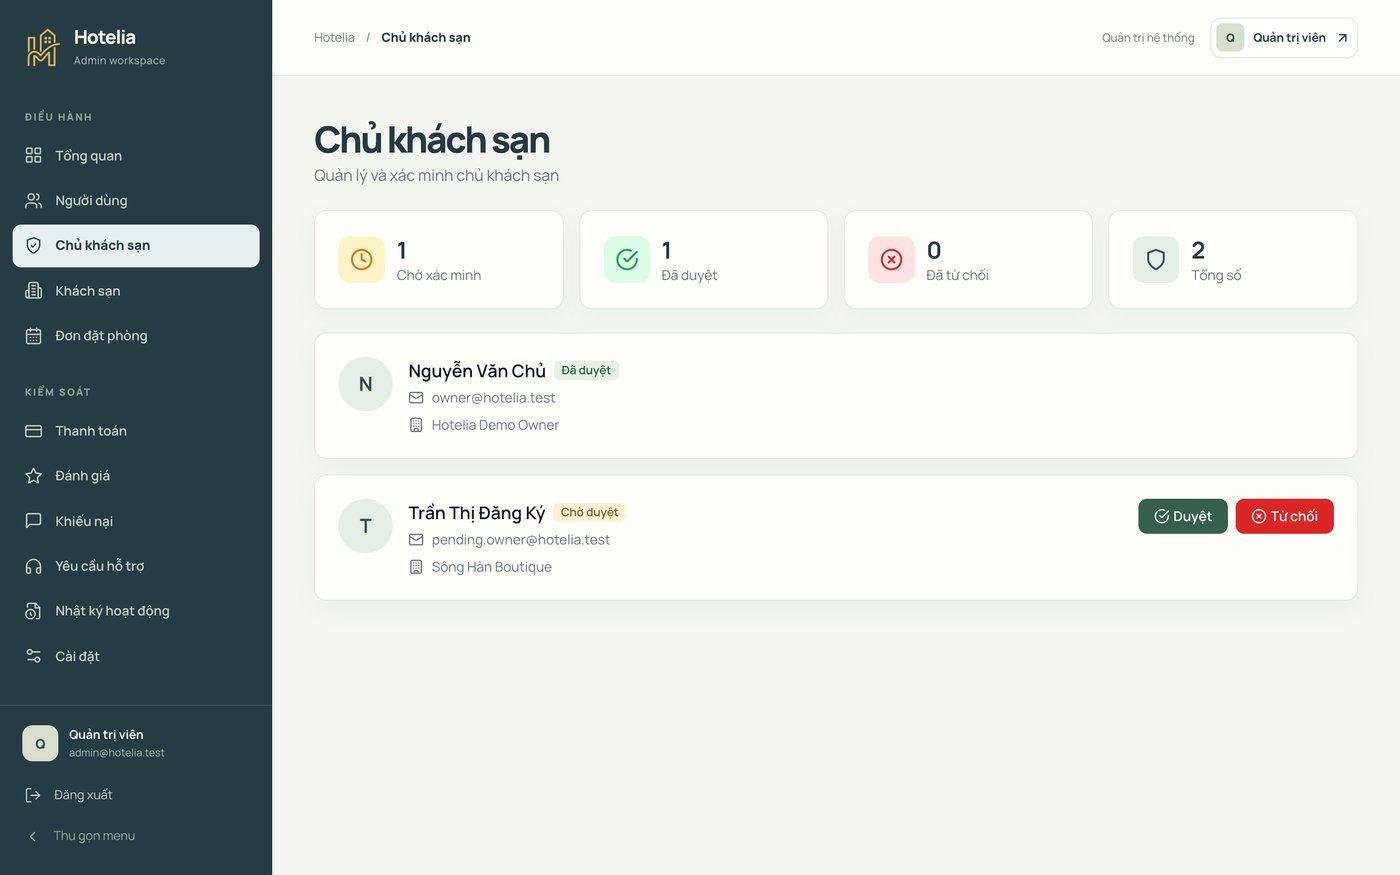
\includegraphics[width=0.49\linewidth]{figures/shots/web-07-admin-owners.jpg}}\\[6pt]
\subcaptionbox{Quản lý khách sạn}{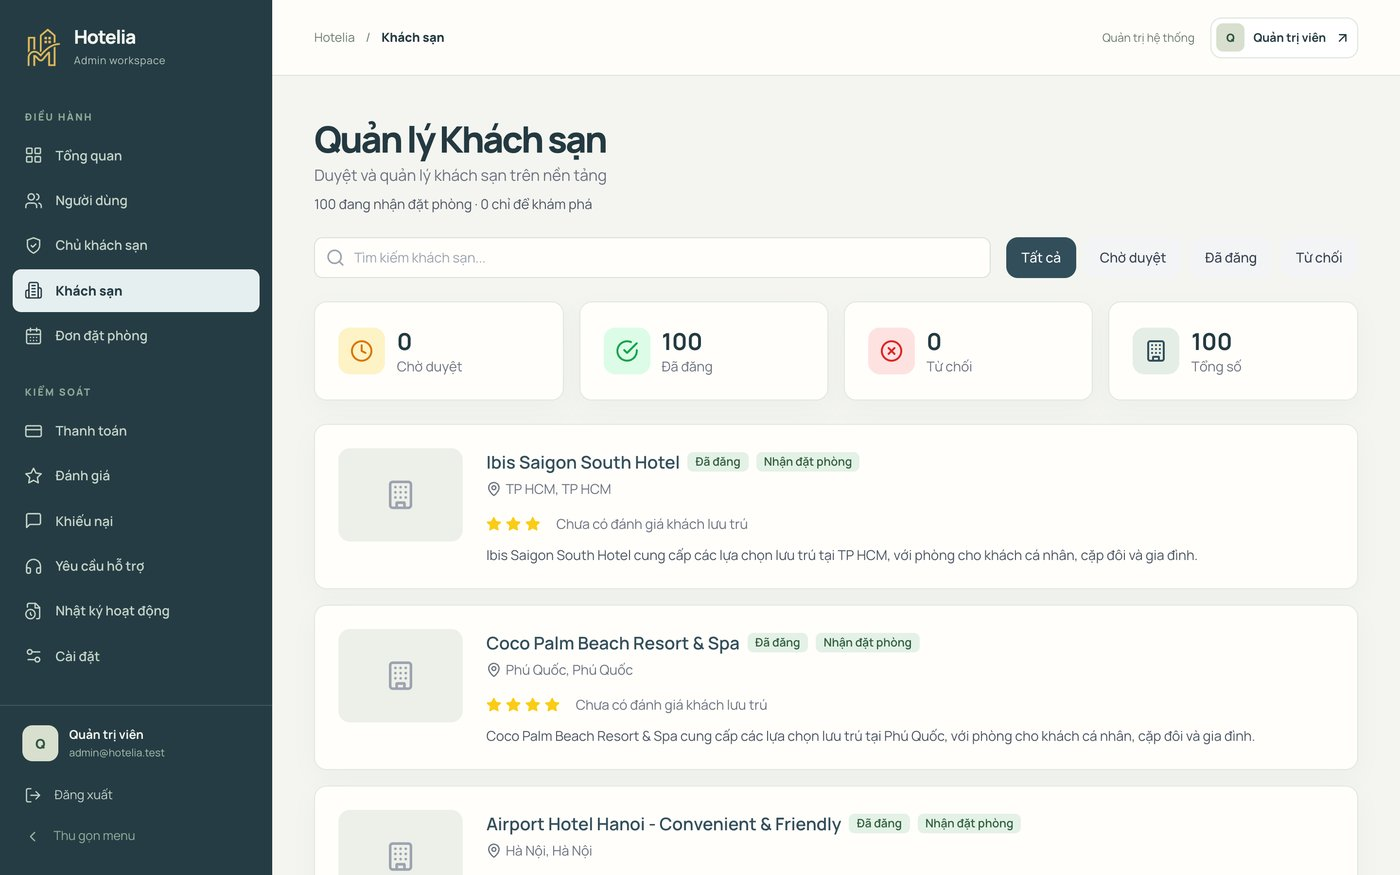
\includegraphics[width=0.49\linewidth]{figures/shots/web-08-admin-hotels.jpg}}\hfill
\subcaptionbox{Quản lý người dùng}{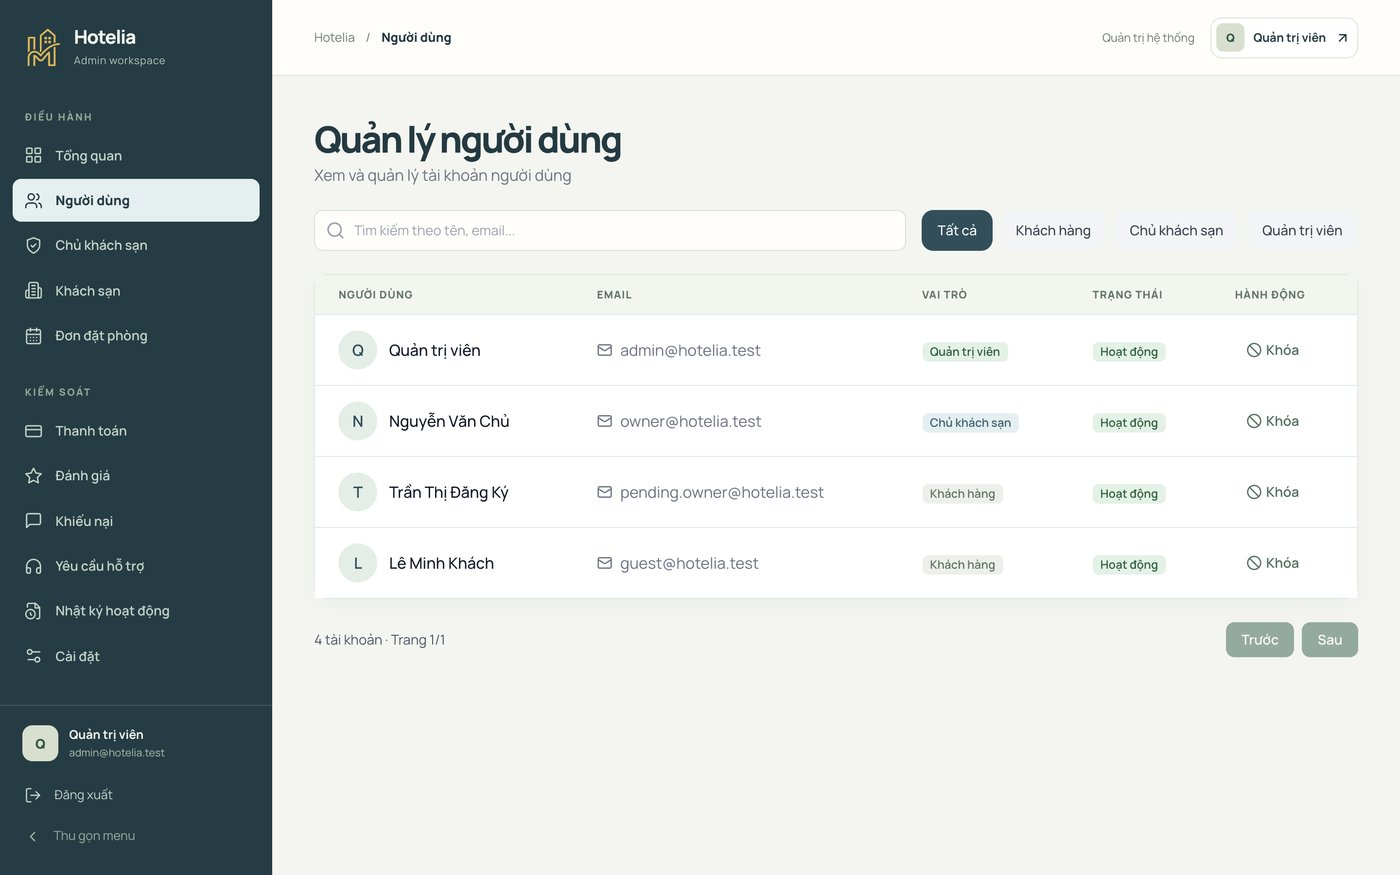
\includegraphics[width=0.49\linewidth]{figures/shots/web-09-admin-users.jpg}}\\[6pt]
\subcaptionbox{Thanh toán}{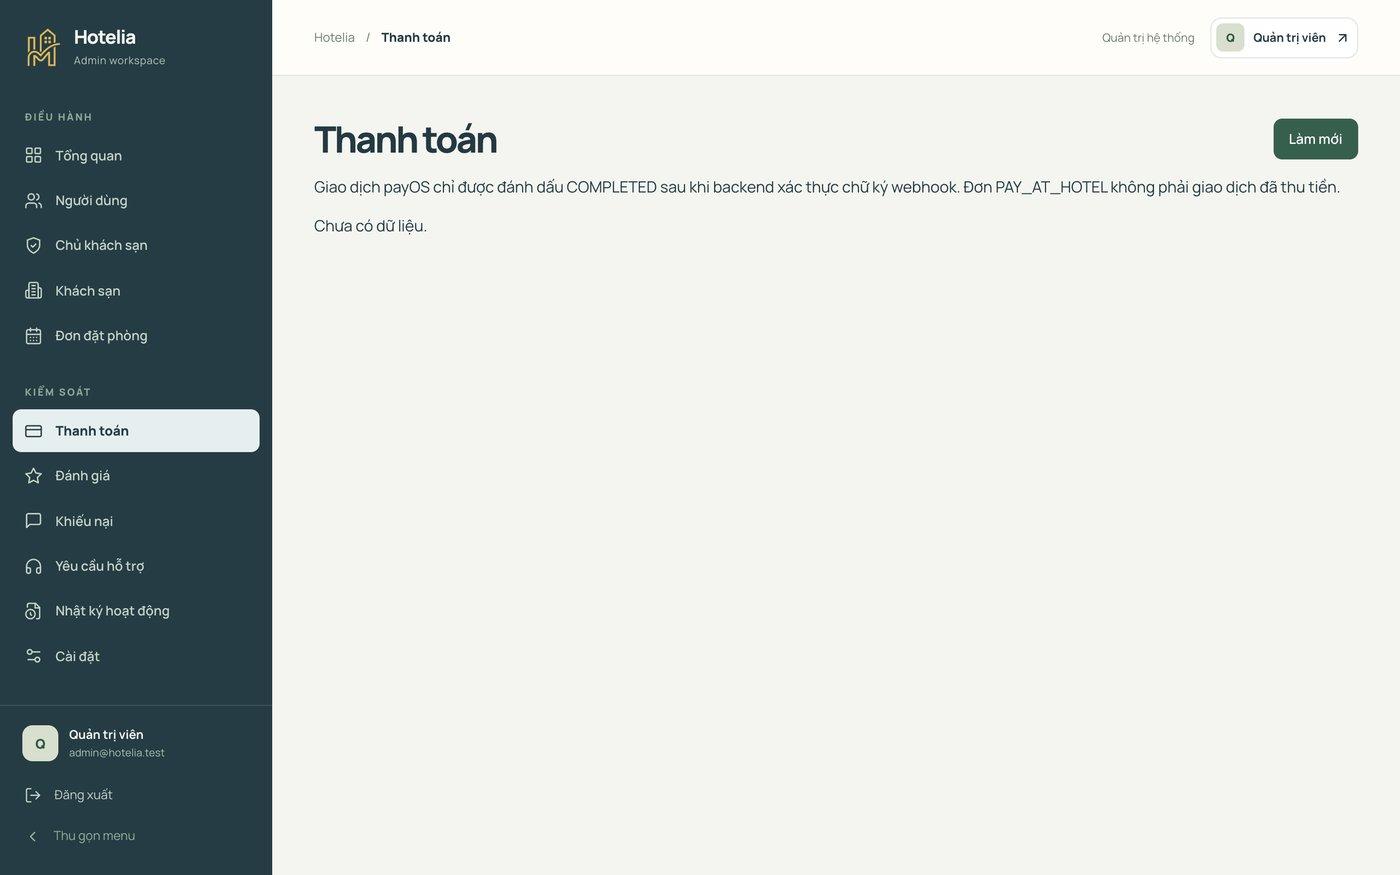
\includegraphics[width=0.49\linewidth]{figures/shots/web-11-admin-payments.jpg}}\hfill
\subcaptionbox{Nhật ký thao tác}{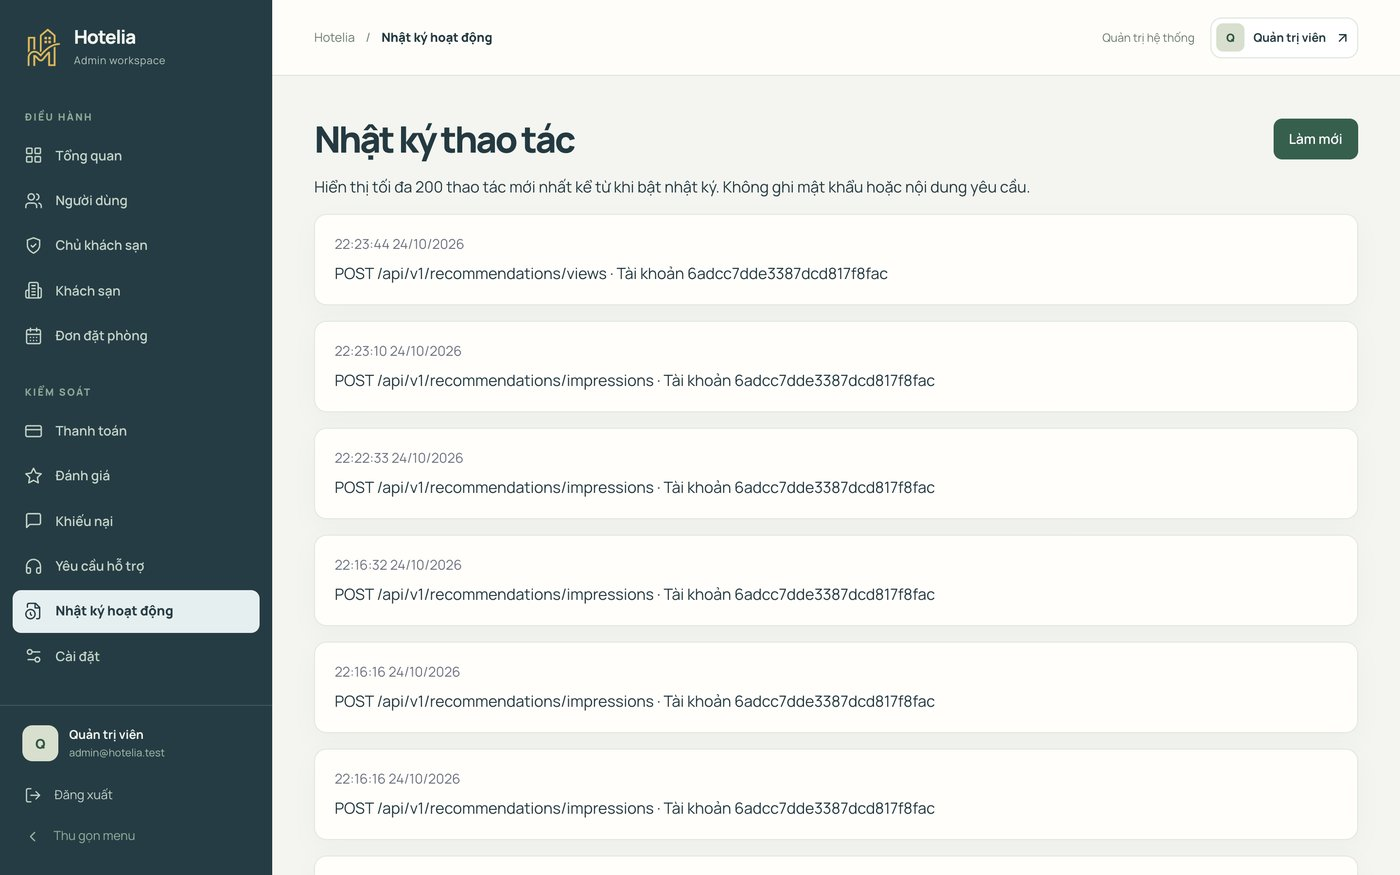
\includegraphics[width=0.49\linewidth]{figures/shots/web-13-admin-audit.jpg}}
\caption{Bảng điều khiển của quản trị viên}\label{fig:web-admin}
\end{figure}

\section{Cài đặt thành phần gợi ý}\label{sec:impl-rec}

\subsection{Đọc và chấm điểm mô hình LightGBM trong NestJS}

Tệp mô hình do LightGBM xuất (\code{dump\_model}) mô tả mỗi cây dưới dạng nút lồng nhau. Nút trong có \code{split\_feature}, \code{threshold}, \code{decision\_type} và \code{default\_left}; nút lá có \code{leaf\_value}. \Cref{lst:tree} là toàn bộ bộ chấm điểm: duyệt từng cây từ gốc tới lá rồi cộng các giá trị lá. Giá trị thiếu (NaN, vô cực) đi theo nhánh mặc định do LightGBM học được. Bộ chấm điểm chỉ chấp nhận phép so sánh \code{<=} (loại duy nhất xuất hiện với đặc trưng số) và ném lỗi với loại khác. Lỗi này khiến hệ thống chuyển sang bộ xếp hạng dự phòng thay vì trả điểm sai.

\lstinputlisting[language=TypeScript, firstnumber=31, caption={Chấm điểm cây LightGBM bằng TypeScript (\code{lightgbm-ranker.ts})}, label={lst:tree}]{code/lgbm-evaluate.ts}

\lstinputlisting[language=TypeScript, firstnumber=108, caption={Nạp và kiểm tra hợp đồng đặc trưng của mô hình}, label={lst:load}]{code/lgbm-load.ts}

Mô hình được nạp một lần khi khởi động (\cref{lst:load}). Nếu tệp thiếu, hỏng, sai danh sách đặc trưng hoặc không có cây, máy chủ ghi cảnh báo và tiếp tục chạy với bộ xếp hạng dự phòng. Tệp \code{nest-cli.json} khai báo \code{recommendations/models/*.json} là tài nguyên cần sao chép vào \code{dist}, để bản build Docker có tệp mô hình.

\subsection{Bảo đảm khớp giữa Python và TypeScript}

Lệch giữa huấn luyện và phục vụ là rủi ro lớn nhất của cách tiếp cận hai ngôn ngữ. Hai cơ chế được dùng để kiểm soát rủi ro này:
\begin{enumerate}
\item Khớp điểm số: tệp mô hình chứa 5 véc-tơ đặc trưng lấy từ tập kiểm tra cùng điểm do LightGBM Python tính. Kiểm thử Jest chấm lại bằng TypeScript và yêu cầu khớp tới 9 chữ số thập phân.
\item Khớp từng đặc trưng: tệp mô hình chứa 2 kịch bản cố định gồm 8 khách sạn thật trong danh mục. Một kịch bản có lịch sử 3 tín hiệu lúc 20:30 thứ Sáu giờ Việt Nam; kịch bản kia không có lịch sử lúc 01:00 thứ Bảy giờ Việt Nam (vẫn là thứ Sáu theo UTC). Kiểm thử Jest tính lại 16 đặc trưng bằng \code{candidateFeatures} và so với giá trị Python tới 9 chữ số thập phân.
\end{enumerate}
Cơ chế thứ hai được bổ sung trong phiên bản v3, sau khi phát hiện hai nguồn lệch ở các phiên bản trước: (i) script huấn luyện tự sinh giá, điểm, số đánh giá bằng hàm băm, khác giá trị máy chủ dùng; (ii) máy chủ tính giờ bằng \code{getHours()} theo múi giờ của tiến trình, trong khi Render chạy theo UTC. Bản sửa (i) thay danh mục sinh bằng ảnh chụp danh mục thật. Bản sửa (ii) tính giờ theo UTC+7 một cách tường minh. Kiểm thử giờ Việt Nam được chạy với \code{TZ=UTC} và \code{TZ=America/Los\_Angeles} để chắc kết quả không phụ thuộc máy chủ. Khi đưa lại mã cũ vào, kiểm thử thất bại như mong đợi.

\section{Triển khai}\label{sec:deploy}

\subsection{Đóng gói máy chủ}

\code{backend/Dockerfile} gồm hai giai đoạn. Giai đoạn \emph{build} trên \code{node:20-alpine} cài đặt phụ thuộc bằng \code{npm ci}, biên dịch TypeScript (\code{nest build} sao chép cả tệp mô hình) rồi loại bỏ phụ thuộc phát triển. Giai đoạn \emph{runtime} chỉ chép \code{package.json}, \code{node\_modules}, \code{dist} và \code{public}, chạy với người dùng \code{node} (không phải root) và có \code{HEALTHCHECK} gọi \code{/health} mỗi 30 giây.

\subsection{Render, Vercel và MongoDB Atlas}

Tệp \code{render.yaml} là bản thiết kế (blueprint) của dịch vụ \code{hotelia-api}: kiểu Docker, gói free, thư mục gốc \code{backend}, đường dẫn kiểm tra sức khỏe \code{/health}, tự triển khai khi có commit. Các biến bí mật (\code{MONGODB\_URI}, \code{CORS\_ORIGINS}, khóa payOS) được khai báo \code{sync: false}, nghĩa là giá trị được nhập trên bảng điều khiển Render và không nằm trong kho mã. \code{JWT\_SECRET} do Render sinh ngẫu nhiên. Bảng điều khiển React được Vercel xây dựng và phục vụ, với \code{vercel.json} chuyển mọi đường dẫn về \code{index.html}.

\Cref{tab:domains} là cấu hình tên miền đo được ngày 24/10/2026 bằng truy vấn DNS và tiêu đề phản hồi HTTP.

\begin{table}[H]
\centering
\caption{Tên miền và nền tảng phục vụ (kiểm tra ngày 24/10/2026)}\label{tab:domains}
\begin{rtable}
\begin{tabular}{|L{3.5cm}|L{4.3cm}|L{6.9cm}|}
\hline
\thead{Tên miền} & \thead{Bản ghi DNS / máy chủ} & \thead{Nội dung đang phục vụ} \\ \hline
api.hotelia.asia & CNAME \code{hotelia-api-eimb.onrender.com}; tiêu đề \code{x-render-origin-server: Render}, \code{server: cloudflare} & API NestJS; \code{/health} trả 200; \code{/api/v1/hotels} trả 100 khách sạn \\ \hline
admin.hotelia.asia & CNAME tới \code{vercel-dns}; \code{server: Vercel} & Bảng điều khiển \code{hotelia-dashboard} \\ \hline
hotelia.asia, www & Bản ghi A/CNAME tới Vercel & Chuyển hướng 308 sang \code{admin.hotelia.asia}, giữ nguyên đường dẫn \\ \hline
\end{tabular}
\end{rtable}
\end{table}

Gói free của Render tạm dừng dịch vụ khi không có lưu lượng. Yêu cầu đầu tiên sau thời gian nghỉ phải chờ khởi động lại: trong lần kiểm tra trên, yêu cầu \code{/health} đầu tiên hết thời gian chờ 20 giây, các yêu cầu sau đó phản hồi bình thường. Đây là giới hạn của gói hạ tầng, được ghi nhận ở \cref{sec:limitations}.

\subsection{Quy trình cập nhật mô hình}

Việc đưa một mô hình mới lên vận hành gồm các bước:
\begin{enumerate}
\item Chạy \code{export\_hotelia\_catalog.py} để lấy ảnh chụp danh mục từ API.
\item Chạy \code{train\_hotelia\_lgb.py} để ghi báo cáo vào \code{research/data/models/} và mô hình vào \code{backend/src/recommendations/models/hotelia-lgbm.active.json}.
\item Chạy kiểm thử Jest (khớp điểm số, khớp đặc trưng, giờ Việt Nam) và pytest.
\item Commit cả ảnh chụp danh mục, báo cáo, mô hình rồi đẩy lên nhánh \code{main}; Render tự xây dựng lại.
\item Kiểm tra \code{GET /api/v1/recommendations}: trường \code{ranking.version} phải bằng phiên bản mới và \code{modelUsed} phải là \code{true}.
\end{enumerate}
Phiên bản v3 được triển khai theo đúng quy trình này ngày 24/10/2026. API chuyển từ \code{hotelia-lgbm-2026-10-23-v1} sang \code{hotelia-lgbm-2026-10-24-v3} khoảng một phút sau khi đẩy mã.

\section{Kết luận chương}

Chương này đã trình bày cài đặt của ứng dụng iOS, máy chủ NestJS, bảng điều khiển React, thành phần gợi ý và cách triển khai. Bốn lỗi được phát hiện và sửa trong quá trình đối chiếu khi viết báo cáo: refresh token dùng được như access token; tràn bố cục ở màn đặt phòng; giao diện không đổi ngôn ngữ ngay; và lệch đặc trưng giữa huấn luyện và phục vụ. \Cref{chap:evaluation} trình bày kết quả kiểm thử các thành phần này.
